\documentclass[a4paper,12pt]{article}
\usepackage{polski}
\usepackage[polish]{babel}
\usepackage[utf8]{inputenc}
\usepackage{helvet}
\usepackage{graphicx}
\usepackage{color}
\usepackage{geometry}
\usepackage{epstopdf}
\usepackage{polski}
\usepackage{hyperref}
\usepackage{url}
\usepackage{indentfirst}
\newenvironment{bottompar}{\par\vspace*{\fill}}{\clearpage}
\geometry{hmargin={2cm, 2cm}, height=10.0in}
\usepackage[toc,page]{appendix}
\addto\captionspolish{%
  \renewcommand{\tablename}{Tabela}%
}

\begin{document}


\thispagestyle{empty}
%% ------------------------ NAGLOWEK STRONY ---------------------------------

\includegraphics[height=37.5mm]{res/agh_logo.pdf}\\
\rule{30mm}{0pt}
{\large \textsf{Wydział Fizyki i~Informatyki Stosowanej}}\\
\rule{\textwidth}{3pt}\\
\rule[2ex]
{\textwidth}{1pt}\\
\vspace{7ex}
\begin{center}
{\LARGE \bf \textsf{Praca magisterska}}\\
\vspace{13ex}
% --------------------------- IMIE I NAZWISKO -------------------------------
{\bf \Large \textsf{Paweł Pęksa}}\\
\vspace{3ex}
{\sf\small Kierunek studiów:} {\bf\small \textsf{Informatyka Stosowana}}\\
\vspace{1.5ex}
{\sf\small Specjalność:} {\bf\small \textsf{Modelowanie i~Analiza Danych}}\\
\vspace{10ex}
%% ------------------------ TYTUL PRACY --------------------------------------
{\bf \huge \textsf{Optymalizacja algorytmów uczenia maszynowego dla niskich statystyk próbek danych}}\\
\vspace{14ex}
%% ------------------------ OPIEKUN PRACY ------------------------------------
{\Large Opiekun: \bf \textsf{dr hab. Marcin Wolter}}\\
\vspace{22ex}
{\large \bf \textsf{Kraków, grudzień 2017}}
\end{center}
%% =====  STRONA TYTUŁOWA PRACY MAGISTERSKIEJKIEJ ====

\newpage

%% =====  TYŁ STRONY TYTUŁOWEJ PRACY MAGISTERSKIEJKIEJ ====
{\sf Oświadczam, świadomy(-a) odpowiedzialności karnej za~poświadczenie nieprawdy, że~niniejszą pracę dyplomową wykonałem(-am) osobiście i~samodzielnie i~ nie korzystałem(-am) ze~źródeł innych niż wymienione w~pracy.}

\vspace{14ex}

\begin{center}
\begin{tabular}{lr}
~~~~~~~~~~~~~~~~~~~~~~~~~~~~~~~~~~~~~~~~~~~~~~~~~~~~~~~~~~~~~~~~~ &
................................................................. \\
~ & {\sf (czytelny podpis)}\\
\end{tabular}
\end{center}

%% =====  TYL STRONY TYTULOWEJ PRACY MAGISTERSKIEJKIEJ ====

\newpage
\rightline{Kraków, ?? grudnia 2017}
\begin{center}
{\bf Tematyka pracy magisterskiej i~praktyki dyplomowej
Pawła Pęksy,
studenta V roku studiów kierunku Informatyka Stosowana, specjalności Modelowanie i~Analiza Danych}\\
\end{center}

Temat pracy magisterskiej:
{\bf Optymalizacja algorytmów uczenia maszynowego dla niskich statystyk próbek danych }\\

\begin{tabular}{rl}

Opiekun pracy:                  & dr hab. Marcin Wolter\\
Recenzenci pracy:               & dr inż. Tomasz Bołd\\
Miejsce praktyki dyplomowej:    & IFJ PAN, Kraków\\
\end{tabular}

\begin{center}
{\bf Program pracy magisterskiej i~praktyki dyplomowej}
\end{center}

\begin{enumerate}
\item Omówienie przedmiotu pracy magisterskiej z opiekunem.
\item Wstępne zapoznanie się z literaturą oraz ramowy plan pracy.
\item Praktyka dyplomowa:
\begin{itemize}
\item przygotowanie oprogramowania i przeprowadzenie wstępnych obliczeń,
\item weryfikacja poprawności obliczeń oraz ewentualna poprawa błędów oprogramowania
\item dyskusja i analiza wyników,
\item sporządzenie sprawozdania z praktyki.
\end{itemize}
\item Kontynuacja obliczeń związanych z tematem pracy magisterskiej.
\item Opracowanie wyników obliczeń oraz przygotowanie odpowiednich tabel oraz wykresów.
\item Analiza wyników, ponowna weryfikacja oraz zatwierdzenie obliczeń przez opiekuna.
\item Opracowanie redakcyjne pracy.
\end{enumerate}


\noindent
Termin oddania w~dziekanacie: ?? grudnia 2017\\[1cm]

\begin{center}
\begin{tabular}{lcr}
.............................................................. & ~~~ &
.............................................................. \\
(podpis kierownika katedry) & & (podpis opiekuna) \\
\end{tabular}
\end{center}

\newpage

\noindent
Na~kolejnych dwóch stronach proszę dołączyć kolejno recenzje pracy popełnione przez~Opiekuna oraz~Recenzenta (wydrukowane z~systemu MISIO i~podpisane przez~odpowiednio Opiekuna i~Recenzenta pracy). Papierową wersję pracy (zawierającą podpisane recenzje) proszę złożyć w~dziekanacie celem rejestracji co najmniej na~tydzień przed planowaną obroną.

\linespread{1.3}
\selectfont

\clearpage
\tableofcontents
\clearpage

\section{Wprowadzenie}\label{intro}
\subsection{Przedmiot pracy}\label{matter}
% http://www.cs.put.poznan.pl/jstefanowski/ml/NEWML_W1lastr.pdf
% https://en.wikipedia.org/wiki/Computational_intelligence#Difference_between_Computational_and_Artificial_Intelligence
% https://books.google.ch/books?hl=en&lr=&id=IZosIcgJMjUC&oi=fnd&pg=PR7&dq=Computational+intelligence&ots=Dwfvy8GnKp&sig=fxvdqBnSEo4YaAU9S3q9XaUUbas#v=onepage&q=Computational%20intelligence&f=false
Uczenie maszynowe jest dziedziną informatyki zajmującą się tworzeniem systemów zdolnych do~uczenia się. Pozwala to na~wykonywanie konkretnego zadania przez~dany system bez konieczności jednoznacznego programowania go. 
Często określane jest jako obszar sztucznej inteligencji lub~też inteligencji obliczeniowej\cite{stefanowski}. Obecnie znajduje zastosowanie w~wielu dziedzinach naszego codziennego życia z~czego często nawet możemy nie zdawać sobie sprawy.
Najpopularniejsze obszary wykorzystania uczenia maszynowego pojawiają się tam, gdzie standardowe algorytmy zawodzą. Wielokrotnie związane jest to tez z~trudnością matematycznego zdefiniowania problemu. 
 Do~tej pory powstało wiele algorytmów, które~pozwalają na~tworzenie programów komputerowych, które~są w~stanie uczyć się na~różne sposoby. Wyróżnia się przede wszystkim dwa podstawowe rodzaje algorytmów uczenia maszynowego:
\begin{itemize}
\item uczenie z nauczycielem (uczenie nadzorowane)
\item uczenie bez nauczyciela (uczenie nienadzorowane).
\end{itemize}
Temat pracy mówi o~uczeniu maszynowym przy niskiej statystyce próbek danych. Implikuje to fakt, ze~autor skupia się na~uczeniu maszynowym z~nauczycielem. W~celu przeprowadzeniu takiego uczenia istnieje potrzeba posiadania danych dzięki którym~dany algorytm stopniowo staje się zdolny do~rozwiązania zadanego mu problemu.
 W~pierwszym momencie mogłoby się zdawać, że~we współczesnym świecie nie spotkamy się już z~tym problemem. Ilość danych składowanych przez~człowieka wzrasta w~tempie eksponencjalnym. W~wielu spotykanych problemach mamy do~czynienia z~danym liczącym tysiące, dziesiątki tysięcy czy~nawet miliony rekordów. Istnieją jednak sytuacje w~których można spotkać się z~postawionym problemem. Wspomnieć można przynajmniej kilka takich dziedzin:
\begin{itemize}
\item medycyna - w tym przypadku możemy mieć do czynienia z sytuacją, kiedy dane pochodzą z pewnego rodzaju badania, które nie zostało do tej pory wykonane na wielu pacjentach i/lub jego wykonanie nie jest proste oraz powszechne
\item specjalistyczne zastosowania biznesowe
\item rzadko występujące zjawiska np. trzęsienia ziemi, powodzie
\item szeregi czasowe  zwłaszcza w sytuacji gdy mamy do czynienia z szeregiem o dużym kroku czasowym.
\end{itemize}

\subsection{Problematyka i cel pracy}
Niniejsza praca przedstawia kilka przykładów, które~obrazują próbę poprawy jakości uczenia maszynowego w~zależności od~ilości dostępnych danych. Testom poddane  zostały następujące algorytmy: sztuczne sieci neuronowe (również z~użyciem uczenia głębokiego - \textit{deep learning}), maszyna wektorów wspierających, drzewo decyzyjnych oraz~las drzew decyzyjnych. W~żadnym wypadku praca nie wyczerpuje zadanego tematu. Autor starał się określić stopień w~którym optymalizacja przy niskiej ilości danych może pomóc w~realizacji konkretnego zadania. W~przypadku 

\subsection{Zawartość dokumentu}
Po~krótkim wprowadzeniu, w~rozdziale \ref{theory}, następuje opis podstaw teoretycznych, które~pozwalają zrozumieć postawione zadanie oraz~proponowane rozwiązania problemu. Rozdział \ref{tools} traktuje o~stworzonych systemach, wykorzystanych narzędziach oraz~organizacji pracy. W~rozdziałach \ref{results} i~\ref{conclusion} przedstawione zostały kolejno wyniki oraz~wnioski wyciągnięte na~podstawie wyników, przeprowadzonych obliczeń oraz~doświadczeń autora zdobytych podczas tworzenia kolejnych systemów uczenia maszynowego.

%źródło: https://medium.com/rants-on-machine-learning/what-to-do-with-small-data-d253254d1a89



\section{Wstep teoretyczny} \label{theory}
W kolejnych podrozdziałach opisane są krótko podstawy teoretyczne dotyczące uczenia maszynowego, wykorzystanych algorytmów oraz użytych metod optymalizacji.
\subsection{Formalny opis uczenia maszynowego}
Uczenie maszynowe okreslane jest jako jedna z galezi sztucznej inteligencji \cite{dnn1}. Formalną definicję podał Tom Mitchell, która brzmi następująco: ,,Mówimy, że maszyna uczy się zadania $T$ w oparciu o doświadczenie $E$ i miarę jakości $P$, jeśli wraz z przyrostem doświadczenia $E$ poprawia się jakość wykonywanego zadania $T$ mierzona przez miarę $P$.''\cite{mitchel} Przykładowo można wymienić trójkę $T$, $E$, $P$ jako diagnozowanie pacjenta na podstawie symptomów, dotychczasowe  liczba wykonanych przez maszynę diagnoz (poprawnie lub nie),  poprawność diagnozowania na podstawie do tej pory niespotkanych przypadków. Powyższe przykłady można mnożyć. Zapis formalny (na podstawie \cite{formal2}) w przypadku algorytmów przedstawionych w nieniejszej pracy możemy przedstawić następująco:
\begin{itemize}
\item $x$ - dane wejściowe algorytmu
\item $y$ - wyjście algorytmu
\item $f$ - funkcja modelowana
\item $g$ - funkcja modelująca.
\end{itemize}
Ogólnie możemy powiedzieć, że zadaniem algorytmu jest znalezienie takiej funkcji $g$, która jak w najlepszy stopniu przybliża funkcję $f$. Odnosząc to do przykładu rozpoznawania chorób, możemy powiedzieć, że modelowaną funkcją jest funkcja symptomów, która przyporządkowuje pacjentowi diagnozę. Uczenie wg danego algorytmu przeprowadza się na podstawie danych:
\begin{equation}
d = (x_1,y_1), (x_2, y_2), ..., (x_n, y_n).
\end{equation}
Każda para $(x_i, y_i)$ stanowi jeden rekord danych lub też jeden przykład podawany do algorytmu. W odniesieniu do przykładu z rozpoznawaniem chorób na podstawie symptomów, jednym rekordem jest konkretny zestaw symptomów ($x_i$) wraz z diagnozą ($y$).  Ogólniej, poszczególne symptomy nazywa się cechami lub atrybutami. W zależności od tego czy $y$ przyjmuje wartości ciągłe czy dyskretne, mamy do czynienia z wykorzystaniem uczenia maszynowego w problemie kolejno regresji lub klasyfikacji. W kolejnych podrozdziałach autor korzysta również z określenia niestabilny algorytm uczenia maszynowego. Mamy z takim do czynienia, gdy mała zmiana w danych wejściowych może spowodować dużą zmianę w predykcjach generowanych przez algorytm\cite{ensamble}.
%W tej pracy wszystkie metody optymalizacji były analizowane pod kątem problemu klasyfikacji lecz naturalne jest ich użycie w przypadku problemu regresji.

\subsection{Wykorzystane algorytmy}
W tym podrozdziale opisane są kolejne algorytmy, które wykorzystywane były w pracy.
\subsubsection{Drzewo decyzyjne}
%www.cs.princeton.edu/courses/archive/spr07/cos424/papers/mitchell-dectrees.pdf
% scikit-learn uses an optimised version of the CART algorithm.
Drzewo decyzyjne jest algorytmem uczenia maszynowego, który może posłużyć w celu rozwiązania problemu klasyfikacji oraz regresji. Funkcja, która jest modelowana przez algorytm przedstawiana jest w formie drzewa matematycznego. Jest to jedna z najpopularniejszych metod, która znalazła swoje wykorzystanie w diagnozowaniu chorób czy ocenie ryzyka kredytowego klientów banków\cite{mitchel}. Zaletami tego podejścia jest między innymi  prostota oraz łatwość interpretacji. Dużą wadą drzew decyzyjnych jest fakt, iż stworzenia optymalnego drzewa decyzyjnego należy do klasy problemów NP-zupełnych. W praktyce tworzenie drzewa oparte jest na metodach heurystycznych\cite{dtscikit}. Na rysunku \ref{dt1image} przedstawione zostało przykładowe drzewo, które mogłoby posłuży do klasyfikacji danych o trzech atrybutach na trzy klasy. Można stwierdzić, że drzewo decyzyjne jest tzw. białą skrzynką (\textit{whitebox}), ponieważ łatwo można zauważyć na jakiej podstawie podjęta została decyzja przyporządkowania do danej klasy.

\begin{figure}[ht!]
\centering
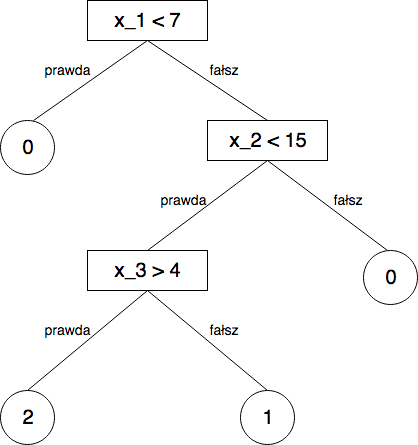
\includegraphics[scale=0.6]{res/dt1.png}
\caption[Caption for LOF]{Przykład drzewa decyzyjnego.\label{dt1image}}
% \caption{Matematyczny model neuronu\label{neuron} Źródło:\footnote{aa} } 
\end{figure} 

\paragraph{Tworzenie drzewa decyzyjnego}\mbox{}\\
%ftp://ftp.boulder.ibm.com/software/analytics/spss/support/Stats/Docs/Statistics/Algorithms/14.0/TREE-CART.pdf
Istnieją różne sposoby na stworzenie drzewa klasyfikacyjnego. Jednym z nich jest algorytm CART -\textit{Classification  and  Regression  Trees}, który był wykorzystany w tej pracy i jest opisany w tym paragrafie. Ideą tego podejścia jest dzielenie danych wejściowych na rozłączne i dopełniające się podzbiory w taki sposób, aby zbiory te pozostawały jak najbardziej jednorodne tj. posiadały jak najwięcej rekordów przynależących do tej samej kategorii. Budowa drzewa zaczyna się od jego korzenia. Wybieramy atrybut wg którego chcemy podzielić dane na dwa jak najbardziej jednorodne zbiory. Po podzieleniu zbioru na dwa podzbioru postępujemy tak samo z następnymi atrybutami. Podział przeprowadzany jest aż do momentu, gdy wszystkie rekordy w każdym podzbiorze przynależą do tej samej kategorii. Należy jednak określić wg których atrybutów dzielić dane tak aby powstawały jak najbardziej jednorodne zbiory. W tym celu wykorzystywane są różnego rodzaju kryteria jednorodności\cite{CART}. Cały algorytm, w uproszczeniu, można opisać w dwóch krokach:
\begin{enumerate}
\item Wybór atrybutu, który pozwoli podzielić zbiór na dwa najbardziej jednorodne podzbiory.
\item Podział wg atrybutu wybranego w kroku 1 jeżeli nie zostały spełnione warunki końca algorytmu\cite{CART}.
\end{enumerate}
Warunkiem końca algorytmu może być sytuacja w której wszystkie stworzone podzbiory są jednorodne lub też moment, gdy dotarliśmy do maksymalnej głębokości drzewa. Każdy podzbiór oznacza kolejną gałąź w drzewie, co powoduje wzrost drzewa. Gdy drzewo jest zbyt duże, staję się ono zbyt skomplikowane i podatne na przeuczenie(\textit{overfitting}). Jednym z parametrów drzewa decyzyjnego, który należy określić jest właśnie jego maksymalna głębokość, która pozwala stworzyć optymalne drzewo. Wspomniany problem przeuczenia został opisany w podrozdziale \ref{problems}. 

\subsubsection{Las drzew decyzyjnych}
%http://jair.org/media/614/live-614-1812-jair.pdf
Las drzew decyzyjnych(\textit{Random forest}) powstał na podstawie idei tworzenia silnego klasyfikatora na podstawie $n$ słabych klasyfikatorów tego samego typu. Podejście to w literaturze określane jest jako \textit{ensable learning}. Szczególnym przypadkiem tego podejścia jest tzw. \textit{bagging}\cite{gonczarek}. Koncepcję \textit{ensable learning} można zobrazować przedstawiając wiele wielomianów, które nie modelują zbyt dobrze funkcji $f$, lecz ich uśrednianie już realizuje to znacznie lepiej, co zostało przedstawione na rysunku \ref{avg1}.  W przypadku uczenia klasyfikatora typu \textit{bagging} tworzymy $m$ klasyfikatorów, każdy z nich uczymy używając $N$ rekordów, który losujemy z powtórzeniami korzystając ze zbioru danych o rozmiarze $N$. Implikuje to fakt, że niektóre ze słabych klasyfikatorów uczone będą na przykładach, które się powtarzają lub niektóre z przykładów w ogóle nie zostaną wzięte pod uwagę. Poszczególne klasyfikatory z pewnością będą cechowały się mniejszą skutecznością jeśli chodzi o klasyfikację, ale ich uśredniony wynik zazwyczaj daje lepsze rezultaty. Wykorzystanie sprawdza się najczęściej w przypadku niestabilnych algorytmów uczenia maszynowego do których zaliczyć też można drzewa decyzyjne\cite{ensable}. Duża zaletą algorytmów typu \textit{bagging} jest fakt, iż ich zrównoleglanie jest bardzo naturalne.
W przypadku lasu drzew decyzyjnych, jak nazwa wskazuje, mamy do czynienia z zespołem słabych klasyfikatorów, które są drzewami decyzyjnymi. Dodatkowo, w celu uczenia poszczególnych drzew, wykorzystujemy tylko $M$ atrybutów zbioru uczącego. Przy czym zaleca się, aby $M=\sqrt{K}$, zakładając, że $K$ oznacza liczbę wszystkich atrybutów zbioru uczącego. Podstawowymi parametrami lasu drzew decyzyjnych, które należy wyznaczyć jest liczba słabych klasyfikatorów wchodzących w skład klasyfikatora oraz maksymalna głębokość wykorzystanych drzew decyzyjnych.
\begin{figure}[ht!]
\centering
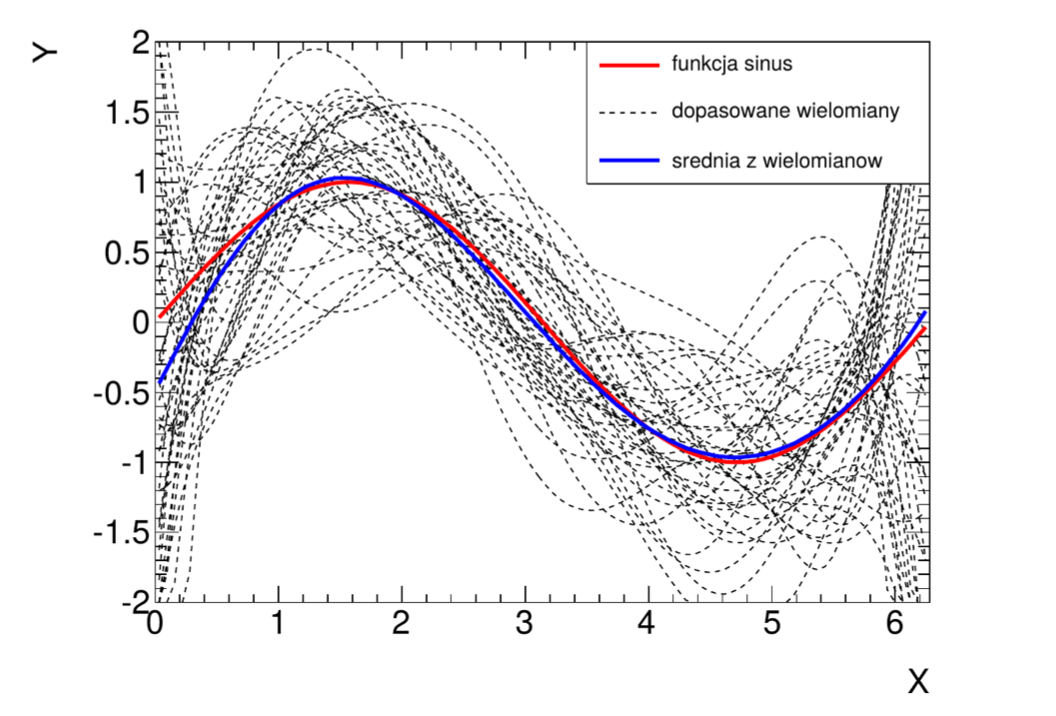
\includegraphics[scale=0.7]{res/avg1.png}
\caption[Caption for LOF]{Ilistracja działania \textit{ensamble learning} TODO:Podać źródło?\label{avg1}}
\end{figure} 

\subsubsection{Maszyna wektorow nosnych}
Maszyna wektorów wspierających (\textit{support vector machine - SVM}) jest modelem matematycznym, który z powodzeniem znajduje swoje zastosowaniu w klasyfikacji oraz regresji. Jej idea jest z jednej strony dość prosta, natomiast z drugiej sprawdza się w dość skomplikowanych problemach\cite{svm1}. Na rysunku \ref{svmIdea} przedstawiona został pomysł, który kryje się za tym algorytmem. Celem jego działania jest znalezienie hiperpłaszczyzny, która dzieli dane wg klas w optymalny sposób. W tym celu, wybierana jest hiperpłaszczyzna, która dzieli dane na dwie klasy zachowując przy tym jak największą odległość od punktów obu tych klas\cite{svm2}. Podstawowa wersja tego algorytmu zapewnia tylko klasyfikacje binarną tzn. taką w przypadku której mamy tylko dwie klasy. W celu rozszerzenia jego działania, istnieją dwa popularne podejścia  tj. \textit{one against one} oraz \textit{one against all}\cite{svm3}. W niniejszej pracy wykorzystane zostało pierwsze z nich, które polega na stworzeniu maszyny wektorów wspierających dla każdej pary klas. Wynika z tego, że konieczne jest stworzenie $K(K-1)/2$ maszyn, zakładając, że $K$ oznacza liczbę atrybutów analizowanego zbioru danych. Ostatecznie, klasa dla konkretnego rekordu danych określana jest poprzez ,,głosowanie''. Ostatnią podstawową kwestią, którą należałoby wyjaśnić, jest pytanie jak \textit{SVM} radzi sobie w przypadku, gdy dane nie są separowalne liniowo, przy których jest również wielokrotnie wykorzystywana. W takiej sytuacji wykorzystana jest transformacja danych, które pozwala na przedstawienie je w przestrzeni w której są one separowalne liniowo. Zobrazowanie tego rozwiązania przedstawia rysunek \ref{svmKernel}. Algorytm dąży do maksymalizacji odległości marginesu, który powstaje podczas dobierania hiperpłaszczyzny (patrz rys \ref{svmIdea}. W wielu przypadkach nie jest możliwe dobranie takiej hiperpłaszczyzny, która dokładnie podzieli dane. Rozwiązaniem w tej sytuacji jest dodanie dodatkowego współczynnika $C$, który dodatkowo uwzględniany jest w procesie optymalizacji. Wartość $C$ stanowi o tym jak duży wpływ na optymalizację mają niepoprawnie sklasyfikowane przykłady w procesie maksymalizacji marginesu i jest jednym z parametrów modelu, który należy wyznaczyć w celu otrzymania najbardziej optymalnego klasyfikatora.

\begin{figure}[ht!]
\centering
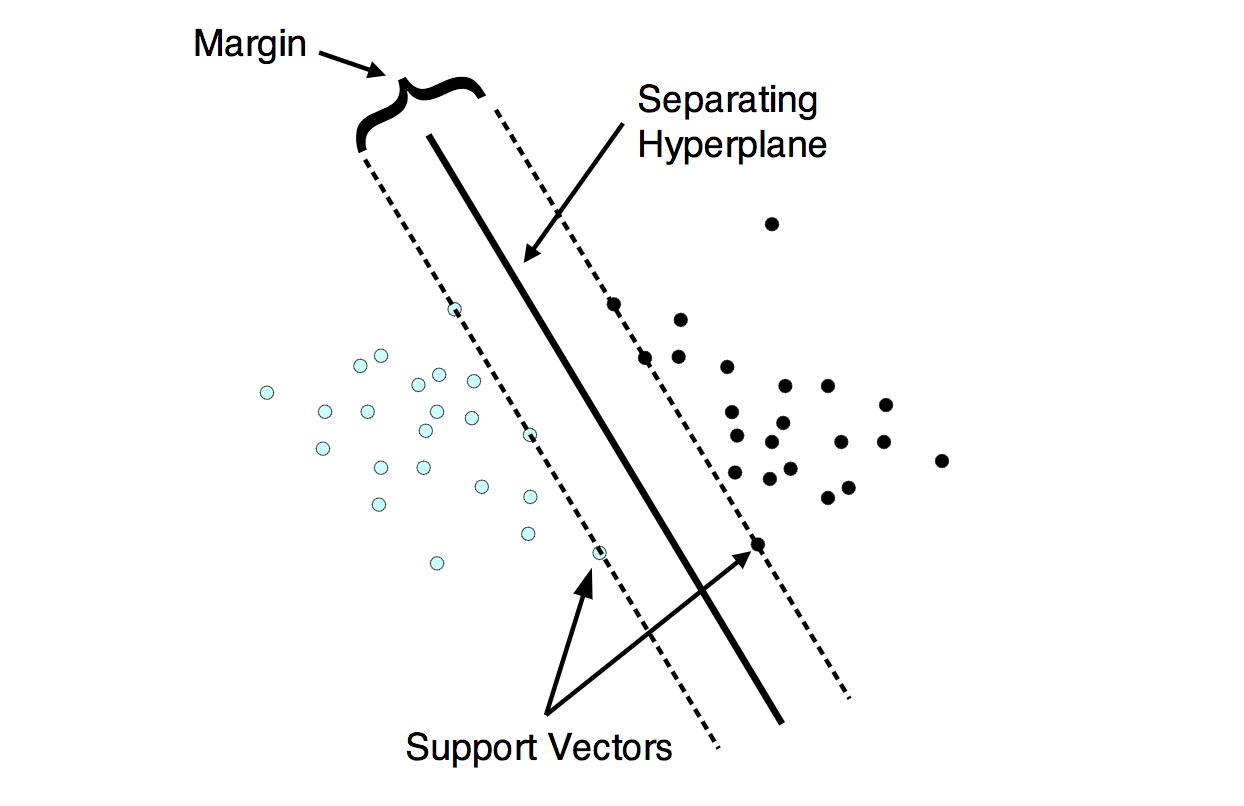
\includegraphics[scale=0.8]{res/svm1.png}
\caption[Caption for LOF]{Rysunek przedstawiający ideę maszyny wektorów wspierających. Źródło:\cite{svm2} \label{svmIdea}}
\end{figure} 

\begin{figure}[ht!]
\centering
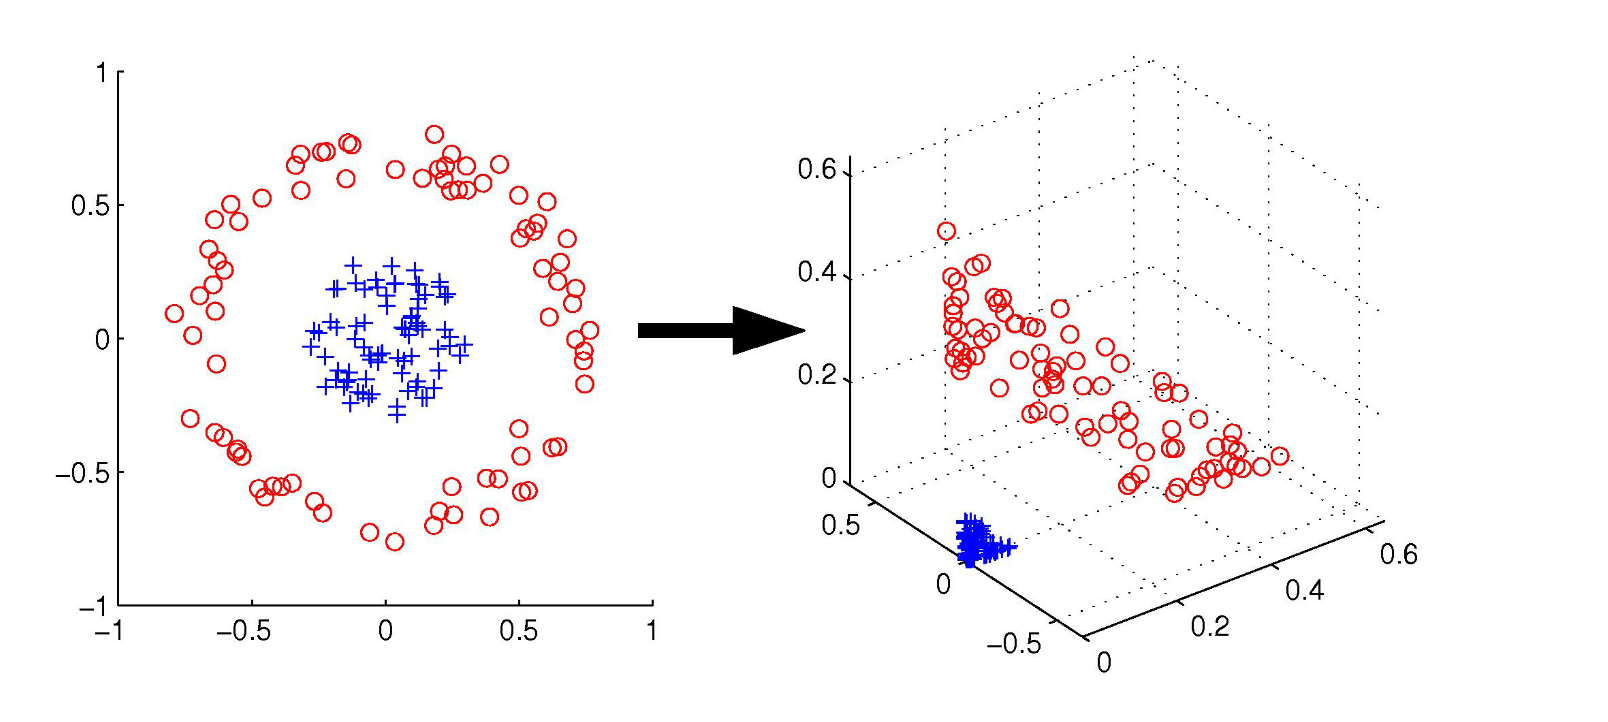
\includegraphics[scale=0.6]{res/svm2.png}
\caption[Caption for LOF]{Rysunek przedstawiający ideę transformowania danych do przestrzeni w której są one liniowo separowalne. Źródło:\cite{svmKernel} \label{svmKernel}}
\end{figure} 

\subsubsection{Tradycyjne sieci neuronowe}
% sieci neuronowe jako blackbox?
Niniejszy podrozdział powstał na podstawie pracy \cite{tadeusiewicz}. Sztuczna sieć neuronowa, dalej nazywana siecią neuronową, jest metodę uczenia maszynowego, którego inspiracją była biologia, a konkretnie ludzki mózg i występujące w nim biologiczne sieci neuronowe. Podstawową odmianą sieci neuronowej jest sieć jednokierunkowa, czyli taka w której nie występują sprzężenia zwrotne. Podstawową jednostką budulcową tego modelu jest neuron, który przedstawiony został na rysunku \label{neuron}. Pojedynczy neuronu wykonuje operację sumy ważonej korzystając z wartości na swoich wejściach oraz wagi przypisanej do każdego wejścia. Wyjście z kolei jest wynikiem zastosowania tzw. funkcji aktywacji na wyniku uprzednio otrzymanym z operacji sumy ważonej. Najpopularniejszymi funkcjami aktywacji w tradycyjnych sieciach neuronowych są funkcja sigmoidalna oraz  tangensoidalna. TODO: I jeszcze moze ta relu?
 
\begin{figure}[ht!]
\centering
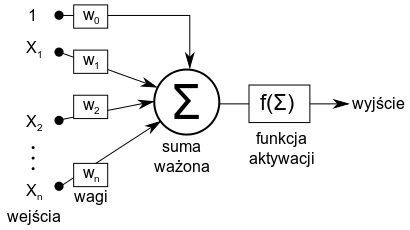
\includegraphics{res/neuron.png}
\caption[Caption for LOF]{TODO:footnotetext on wrong page Matematyczny model neuronu\label{neuron}\footnotemark}
% \caption{Matematyczny model neuronu\label{neuron} Źródło:\footnote{aa} } 
\end{figure} 
\footnotetext{\url{http://pl.wikipedia.org/wiki/Plik:
Neuron_McCullocha-Pittsa.png}}


Cała sieć neuronowa jest niczym innym niż połączonymi ze sobą neuronami. Każdemu połączeniu przypisana jest waga liczbowa, która informuje o tym jak wpływają na siebie poszczególne komórki sieci. Wszystkie neurony zgrupowaną są w warstwy z których możemy wyróżnić:
\begin{itemize}
\item warstwę wejściową
\item jedną lub więcej warstw ukrytych
\item warstwę wyjściową
\end{itemize}

W każdej warstwie może znajdować się dowolna ilość neuronów. Przykład sieci neuronowej został przedstawiony na rysunku \label{net}.

\begin{figure}[ht!]
\centering
% obrazek pobrany z 
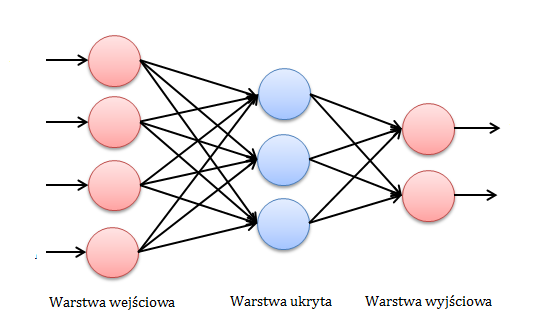
\includegraphics{res/exampleNet.png}
\caption[Caption for LOF]{Przykładowa jednokierunkowa sieć neuronowa\label{net}\footnotemark} 
\end{figure}

\footnotetext{\url{https://2ml4pa.bn1303.livefilestore.com/y2p6no6Dn0weHW3FG9tceTUS9lohx5ldcxvFZRhKdbeFQi2kntad_77gKeKIC-INcsFRCvGI-_DY9lMdZzaX8jkSHDvqlcT3qRnftpAt7esi4s/1.PNG?psid=1}}

W każdej iteracji uczenia sieci, na wejście podawany są dane. W zależności o odpowiedzi otrzymanej przez sieć przeprowadzana jest poprawa wag. Po przeprowadzeniu uczenia, sieć powinna ustalić wagi takie, aby poprawnie odpowiadać na kolejne sygnały wejściowe. W ogólności mówimy o minimalizacji błędu sieci $Q$ w zależności od wag sieci. W równaniu aktualizującym wagi występuję również współczynnik $\eta$, który jest tzw. współczynnikiem uczenia, który zmniejsza wprowadzane poprawy wag sieci. Dzięki temu współczynnikowi proces uczenia przebiega bardziej optymalnie. Jest on jednym z parametrów modelu, który należy wyznaczyć. Kolejnym z parametrów tego modelu jest liczba neuronów w warstwie ukrytej. Liczba neuronów w warstwie wejściowej zależy od liczby atrybutów naszych danych, natomiast wyjściowej od tego na ile kategorii dane są klasyfikowane. Pierwsze algorytmy uczenia, które powstały potrafiły przeprowadzić uczenie sieci neuronowej tylko o jednej warstwie. W celu uczenia sieci wielowarstwowych powstał algorytm wstecznej propagacji. Błąd dla poszczególnych neuronów jest w tym algorytmie obliczany ,,od przodu'' to znaczy zaczynając od warstwy wyjściowej. Dla neuronów w warstwie ukrytej błąd obliczany jako średnia ważona błędów neuronów do których dany neuron wysłał swój sygnał.
\subsubsection{Głębokie sieci neuronowe}
Niniejszy rozdzial zostal napisany na podstawie\cite{dnn1}.\\
% https://stats.stackexchange.com/questions/182734/what-is-the-difference-between-a-neural-network-and-a-deep-neural-network
% https://arxiv.org/pdf/1703.09039.pdf
Ideą stojącą za głębokimi sieciami neuronowymi jest tworzenie sieci, które posiadają wiele warstw ukrytych. Wiele, to znaczy od kilku do nawet kilku tysięcy. W tradycyjnych sieciach neuronowych zazwyczaj występowało co najwyżej kilka warstw ukrytych, a bardzo często tylko jedna. Udowodnione zostało matematycznie, że sieć o takiej strukturze jest zdolna do modelowania jakiejkolwiek funkcji pod warunkiem występowania w niej nieliniowych funkcji aktywacji w neuronach. W przypadku tradycyjnych sieci neuronowych na wejście sieci podawane są atrybuty, które należy samemu określić. Są to wyznaczone matematycznie cechy w zależności od problemu. Przykładem takiej sytuacji możesz być rozpoznawanie konkretnych obiektów na obrazie. Do sieci neuronowej możemy podać w takiej sytuacji konkretnie wyliczone cechy obrazu zamiast przekazywać wartość każdego piksela, co powodowałoby, że sieć miałaby bardzo dużo wejść, a co za tym idzie, trudno byłoby ją nauczyć. Takimi cechami mogą być np. jasność obrazu, tekstura, wskaźnik występujących na obrazie linii lub okręgów oraz wiele więcej. Przy operacji ekstrakcji cech z obrazu następuję naturalnie pewna utrata informacji. W przypadku głębokich sieci neuronowych nie dokonujemy ekstrakcji cech co jest zasadniczą różnicą. Na wejście sieci podawany są dane w stanie ,,surowym''. Pozwala to na uniknięcie utraty informacji co przy odpowiedniej ilości danych oraz dobrze zbudowanej sieci pozwala na znacznie lepsze wyniki. Sieć podczas procesu uczenia jest w stanie sama nauczyć się jakie cechy powinna rozpoznawać. Różnica ta została zilustrowana na rysunku \ref{dnnDiff}.

\begin{figure}[ht!]
\centering
% obrazek pobrany z 
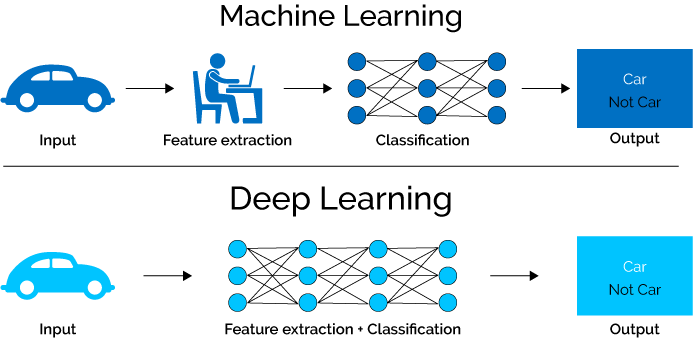
\includegraphics[scale=0.5]{res/dnn1.png}
\caption[Caption for LOF]{Różnica tradycyjnych sieci neuronowych oraz głębokich sieci neuronowych w kontekście ekstrakcji cech\label{dnnDiff}\footnotemark} 
\end{figure}
\footnotetext{\url{https://hackernoon.com/log-analytics-with-deep-learning-and-machine-learning-20a1891ff70e}}

\subsubsection{Konwolucyjne sieci neuronowe}
Niniejszy rozdział został napisany na podstawie\cite{nielsen}.\\
Konwolucyjne sieci neuronowe są najpopularniejszym typem głębokich sieci neuronowych. Znajdują swoje zastosowanie wszędzie, gdzie możemy zetknąć się z potrzebą analizy obrazów. Ich nazwa wynika wynika z faktu, iż bazują one na operacji konwolucji. W przypadku tradycyjnych sieci neuronowych, w sytuacji analizy obrazu bez ówczesnej ekstrakcji cech, należałoby podać na każde wejście sieci wartość pojedynczego piksela. Problemem tego podejścia jest to, że nie jest brana pod uwagę przestrzenna natura obrazu. Każde wejście sieci traktowane jest indywidualnie i nie jest ważne jego położenie na obrazie.  Konwolucyjne sieci neuronowe wykorzystują przestrzenną naturę obrazu. Ich architektura jest do tego dostosowana. Głównymi elementem sieci tego typu odróżniającymi je od tradycyjnych jest istnienie warstw konwolucyjnej. W przypadku tradycyjnych sieci neuronowych, zazwyczaj wyobrażamy sobie warstwę jako pojedyncza linie neuronów. Dla warstwy konwolucyjnej, bardziej naturalne jest jej przedstawienie w dwóch wymiarach.
\begin{figure}[ht!]
\centering
% obrazek pobrany z 
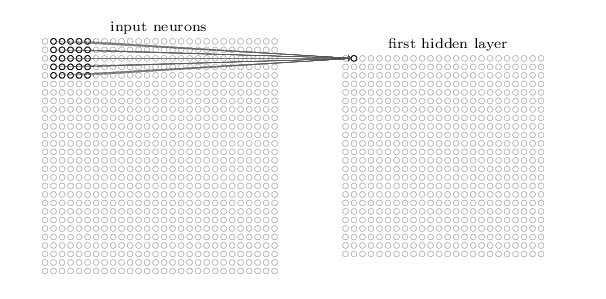
\includegraphics[scale=0.6]{res/cnn1.png}
\caption[Caption for LOF]{Warstwa wejściowa konwolucyjnej sieci neuronowej przedstawiona w dwóch wymiarach. Źródło:\cite{nielsen}\label{cnn1}} 
\end{figure}

Wartością każdego neuronu wejściowego jest wynik operacji konwolucji. W celu otrzymania wszystkich wejść należy ,,przesuwać'' maskę po całym obrazie. W zależności od rozmiaru maski (zazwyczaj $3x3$, $5x5$ lub $7x7$) otrzymujemy odpowiednią liczbę wejść sieci. Operacja ta została przedstawiona na rysunku \ref{cnn1}. Należy wspomnieć, że wagi wszystkich neuronów są wspólne. Można stwierdzić, że w ten sposób pierwsza warstwa służy do wykrycia dokładnie jednej cechy obrazu. Jedna cecha na jedną warstwę, to byłoby jednak za mało, więc ostatecznie najlepiej przedstawić pojedyncza warstwę konwolucyjną w trzech wymiarach, co można zobaczyć na rysunku \ref{cnn2}.

\begin{figure}[ht!]
\centering
% obrazek pobrany z 
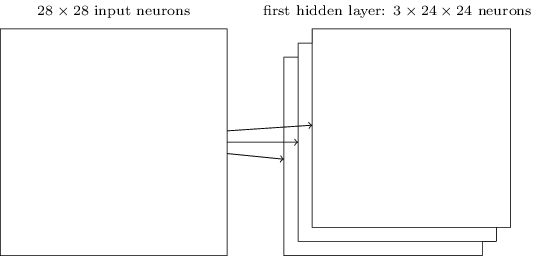
\includegraphics[scale=0.6]{res/cnn2.png}
\caption[Caption for LOF]{Warstwa wejściowa konwolucyjnej sieci neuronowej przedstawiona w trzech wymiarach. Źródło:\cite{nielsen}\label{cnn2}} 
\end{figure}

W sieciach konwolucyjnych, oprócz warstw konwolucyjnych, występują także warstwy typu \textit{pooling}, które pozwalają na pomniejszenie obrazu, co z kolei redukuje w pewnym stopniu koszty związane z obliczeniami. Jedną z podstawowych wykorzystywanych technik jest tzw. \textit{max-pooling}. Ponownie używając maski dowolnego rozmiaru (zazwyczaj $2x2$) ,,przechodzimy'' po całym obrazie, lecz tym razem wybierając do warstwy po operacji \textit{poolingu} piksel o najwyższej wartości.

\begin{figure}[ht!]
\centering
% obrazek pobrany z 
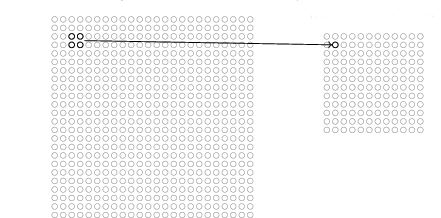
\includegraphics[scale=0.6]{res/pooling.png}
\caption[Caption for LOF]{Warstwa typu \textit{pooling}. Źródło:\cite{nielsen}\label{pooling}} 
\end{figure}

Po warstwach konwolucyjnych oraz typu \textit{pooling}, których ilość jest arbitralna, następuję przejście do tradycyjnych sieci neuronowych, gdzie dokonywana jest ostateczna klasyfikacja. Cała architektura przedstawiona została na rysunku \ref{cnn3}.

\begin{figure}[ht!]
\centering
% obrazek pobrany z https://www.kernix.com/blog/a-toy-convolutional-neural-network-for-image-classification-with-keras_p14
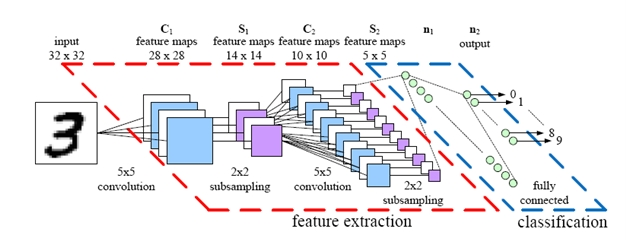
\includegraphics[scale=0.75]{res/cnn3.jpg}
\caption[Caption for LOF]{Architektura konwolucyjnych sieci neuronowych\footnotemark\label{cnn2}} 
\end{figure}
\footnotetext{\url{ https://www.kernix.com/blog/a-toy-convolutional-neural-network-for-image-classification-with-keras_p14}}

\subsection{Wykorzystane metody optymalizacji}
\subsubsection{Walidacja krzyzowa - wyznaczanie parametrow modelu}
\subsubsection{Sztuczne powiekszanie zbioru danych}
\subsubsection{Ekstrakcja cech}
\subsection{Problemy wynikające z niskiej ilości danych?}\label{problems}
\subsection{Proponowane rozwiązania?}
\paragraph{LDA}
\paragraph{PCA}


\section{Wykorzystane narzędzia i technologie} \label{tools}
W~celu przeprowadzenia zaproponowanych eksperymentów należało wybrać język programowania wraz z~odpowiednimi bibliotekami zapewniającymi należyte funkcjonalności. Niniejszy rozdział traktuje o~technologiach wybranych w~celu realizacji postawionych zadań.
\subsection{Język programowania oraz biblioteki programistyczne}
Językiem programowania, który~został wybrany do~realizacji wszystkich zadań w~tej pracy został język Python będący językiem wysokiego poziomu. Jest to obecnie jeden ze~standardów w~świecie inżynierii komputerowej obok takich rozwiązań jak~np. pakiet obliczeniowy Matlab, który~jednak nie jest rozpowszechniany na~licencji \textit{open-source}. Mogłoby się wydawać na~początku, biorąc pod~uwagę, że~jest to język skryptowy, że~działanie stworzonych programów przy jego użyciu będzie skutkowało względnie wysokim czasem wykonania. Istniejące jednak moduły takie jak~NumPy czy~SciPy\cite{scipy} zaimplementowane są w~języku C dzięki czemu, pomimo łatwości tworzenia nowego kodu, nie tracimy jeśli chodzi o~szybkość działania. Dodatkowo, razem z~wymienionymi pakietami, powszechnie wykorzystywana jest biblioteka Matplotlib\cite{matplotlib} zapewniająca funkcjonalności związane z~rysowaniem wykresów. Istnieje również duża społeczność skoncentrowana wokół języka Python dzięki czemu rozwiązywanie napotkanych problemów jest dużo prostsze. Oprócz wspomnianych pakietów, wykorzystane również zostały biblioteki bezpośrednio związane z~uczeniem maszynowym:
\begin{itemize}
\item Scikit-Learn\cite{scikit} - algorytmy uczenia maszynowego oraz pokrewne (np. związane z~ekstrakcją cech),
\item TensorFlow\cite{tensorflow} - algorytmy uczenia maszynowego wraz z głębokimi sieciami neuronowymi,
\item Keras\cite{keras} - nakładka na pakiet TensorFlow, wykorzystany w pracy w celu obróbki obrazów,
\item HyperOpt\cite{hyperopt} - optymalizacja parametrów algorytmów uczenia maszynowego.
\end{itemize}
Kolejną znaczącą zaletą języka Python jest bogata biblioteka standardowa. Do~stworzenia odpowiednich programów posłużono się między innymi modułami odpowiedzialnymi za~wielowątkowość czy~logowanie zdarzeń mających miejsce w~trakcie wykonania programu. Obok języka Python wykorzystany został bash, który~jest najpopularniejszą powłoką sytemu UNIX. Pozwalało to na~uruchomienie wielu skryptów jednocześnie z~różnymi parametrami (także równolegle). W~niektórych przypadkach w~celu tworzenia wykresów zamiast biblioteki Matplotlib wykorzystany został pakiet Gnuplot ze~względu na~komfort jego użycia. Całość zarządzana była przy użyciu rozproszonego systemu kontroli wersji Git.

\subsection{Środowisko}
Dzięki uprzejmości Instytutu Fizyki Jądrowej PAN w~Krakowie wszystkie obliczenia przeprowadzone zostały w~chmurze obliczeniowej CC1\cite{cc1Article}, co zapewniało znacznie większą moc obliczeniowej niż w~przypadku użycia komputera osobistego, a~także wygodę jeśli chodzi o~zarządzanie systemem oraz~danymi. Najmocniejsza możliwa konfiguracja dla nowo-utworzonej maszyny w~chmurze CC1 charakteryzowała się posiadaniem 12 wirtualnych procesorów oraz~19,6~GB pamięci RAM i~była, w~miarę dostępności, najczęściej używana. Obliczenia przeprowadzane zostały pod~systemem operacyjnym Linux z~użyciem dystrybucji Ubuntu. Python jest językiem przenośnym, także nie byłoby problemów z~użyciem systemu Windows, lecz wykorzystanie systemu Linux było bardziej komfortowe z~punktu widzenia programisty.


\section{Przeprowadzone eksperymenty} \label{results}
Niniejszy rozdział opisuje przeprowadzone eksperymenty w~ramach których autor starał się ocenić jak~bardzo sprawdzane metody są w~stanie pomóc w~uzyskaniu wyższej skuteczności w~przypadku uczenia maszynowego. 

\subsection{Sztuczne powiększanie zbioru danych}
\subsubsection{Opis problemu}
Eksperyment sztucznego powiększania danych został przeprowadzony w~oparciu o~konkurs ,,Dogs vs. Cats'' opublikowany w~serwisie Kaggle.\footnote{\label{myfootnote1}\url{https://www.kaggle.com/c/dogs-vs-cats}} Zadaniem uczestników było stworzenie systemu, który~jest w~stanie rozwiązać problem rozpoznawania psów i~kotów na~obrazie. Udostępniona została baza danych 25000 sklasyfikowanych obrazów o~różnych rozmiarach. Mały wycinek udostępnionych danych został przedstawiony na~rysunku \ref{catsdogs}. W~celu ewaluacji stworzonego modelu udostępniony był zbiór 12500 niesklasyfikowanych obrazów. Najlepsze rezultaty uczestnicy otrzymywali przy użyciu głębokich sieci neuronowych i~także ta metoda została wykorzystana w~tej pracy. Zwycięzca pierwszej edycji konkursu uzyskal skuteczność 98,9\%\footnote{\label{myfootnote2}\url{https://plus.google.com/+PierreSermanet/posts/GxZHEH9ynoj}} korzystając właśnie z~głębokich sieci neuronowych. Autor najlepszego rozwiązania, oprócz posłużenia się całym zbiorem opublikowany przez~serwis Kaggle, dodatkowo wykorzystał inny zbiór danych~-~ILSVRC12\footnote{\url{http://www.image-net.org/challenges/LSVRC/2012/results.html}} - w~celu wstępnego uczenia sieci, co daje dobrą podstawę do~treningu modelu dla docelowego zadania. W~przeprowadzonych obliczeniach, dotyczących niniejszej pracy, nie został jednak wykorzystany cały zbiór ze~względu na~bardzo długi czas wykonania programu. Celem tego eksperymentu było zbadanie poprawy klasyfikacji przy użyciu sztucznego powielania danych. Uczenie sieci przeprowadzone zostało przy użyciu 8000 obrazów, a~z kolei 1000 obrazów przeznaczone zostało do~testowania, co w~żadnym wypadku nie stanowi przeszkody w~osiągnięciu założonego celu tego eksperymentu. Pojedyncze uczenie, wraz~z ewaluacją, trwało około 17 godzin. Każdy obraz podawany do~sieci był 4 razy, co dawało 32000 iteracji przy pojedynczym uczeniu. Dla uzyskania statystyki, ze~względu na~zmienne losowe występujące w~tej metodzie, uczenie oraz~testowanie systemu przeprowadzane było w~każdym przypadku 5 razy. Najprościej ujmując, całe postępowanie można opisać w~dwóch krokach. Pierwszym z~nich było uczenie oraz~testowanie systemu przy użyciu oryginalnych obrazów. Drugim natomiast, uczenie oraz~testowanie przy wykorzystywaniu nieco zmodyfikowanych obrazów. W~kroku drugim jednak, można również wyszczególnić dwa podejścia:
\begin{itemize}
\item statyczne powielanie obrazów,
\item dynamiczne powielanie obrazów.
\end{itemize}
Statyczne generowanie obrazów polega na~stworzeniu nowych, zmodyfikowanych obrazów przed uruchomieniem programu. Można określić liczbę obrazów, którą~chcemy stworzyć dla każdego obrazu oryginalnego, następnie wygenerować docelowe obrazy, aby~ostatecznie użyć ich do~uczenia sieci neuronowej. W~przypadku dynamicznego generowania obrazów, sama generacja wykonywana jest w~trakcie działania programu za~każdym razem gdy sieć potrzebuje danych. Przy uwzględnieniu wystarczającej ilości zmiennych losowych zapewnia to, że~z~bardzo dużym prawdopodobieństwem nie zostaną wykorzystane do~uczenia dokładnie dwa takie same obrazy, więc można oczekiwać w~tym przypadku lepszych wyników. Jego wadą jednak, jest fakt, iż~za każdym uruchomieniem programu, na~bieżąco wykonywana jest generacja nowych obrazów, co jest narzutem obliczeniowym. To podejście zostało ostatecznie wykorzystane w~niniejszej pracy ze~względu na~swoje zalety. W~przypadku statycznego generowania obrazów, przed każdym uruchomieniem programu należałoby obliczyć, ile obrazów należy wygenerować, tak, aby~żaden z~nich nie został podany do~sieci dwa razy.

\begin{figure}[ht!]
\centering
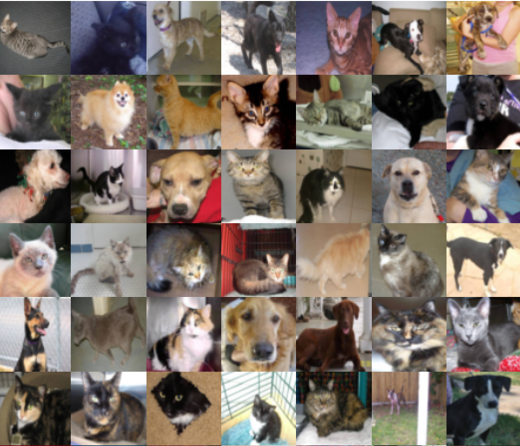
\includegraphics[scale=0.8]{res/catsdogs.png}
\caption[Caption for LOF]{Przykładowe zdjęcia z bazy danych serwisu Kaggle dla konkursu ,,Dogs vs. Cats'' \label{catsdogs}}
\end{figure} 

\subsubsection{Stworzone rozwiązanie}
System stworzony w~przypadku tego eksperymentu składał się z~dwóch głównych komponentów. W~celu wyodrębnienia wczytywania oraz~generowania danych stworzony został komponent nazwany DataProvider, który~pozwalał w~zręczny sposób podawać dane do~sieci. Drugim komponentem była sama sieć neuronowa. Ze~względy jednak na~duże wymogi obliczeniowe w~przypadku uczenia, możliwości dobrania odpowiedniej architektury oraz~optymalizowania parametrów były dość ograniczone. Wszystkie wykorzystywane obrazy zostały zmniejszone do~rozmiarów 64x64. Ostatecznie dobrana architektura sieci zawierała trzy warstwy konwolucyjne, jedną warstwę typu \textit{max pooling}, jedną warstwę w~pełni połączoną  oraz~jedną warstwę wyjściową. Warstwa wyjściowa składała się z~dwóch neuronów odpowiednio dla dwóch rozpoznawanych klas. W~przypadku warstw konwolucyjnych, wszystkie posiadały po~64 filtry z~tym, że~w~pierwszych dwóch stosowana była maska o~rozmiarach 7x7, a~w trzeciej 5x5.  Warstwa w~pełni połączona zawierała 512 neuronów. Obrazy generowane były dynamicznie podczas działania programu. Zastosowane zostały następujące operacje:
\begin{itemize}
\item rotacja obrazu w zakresie od 0 do 40 stopni,
\item przesunięcie w poziomie o długość do 20\% szerokości obrazu,
\item przesunięcie w pionie o długość do 20\% wysokości obrazu,
\item odbicie lustrzane obrazu w poziomie,
\item przybliżenie obrazu do 20\%.
\end{itemize}
Na~rysunku \ref{catdogsimages} został przedstawiony obraz oryginalny oraz~cztery obrazy wygenerowane na~jego podstawie zgodnie z~powyższymi parametrami.

\begin{figure}[ht!]
\centering
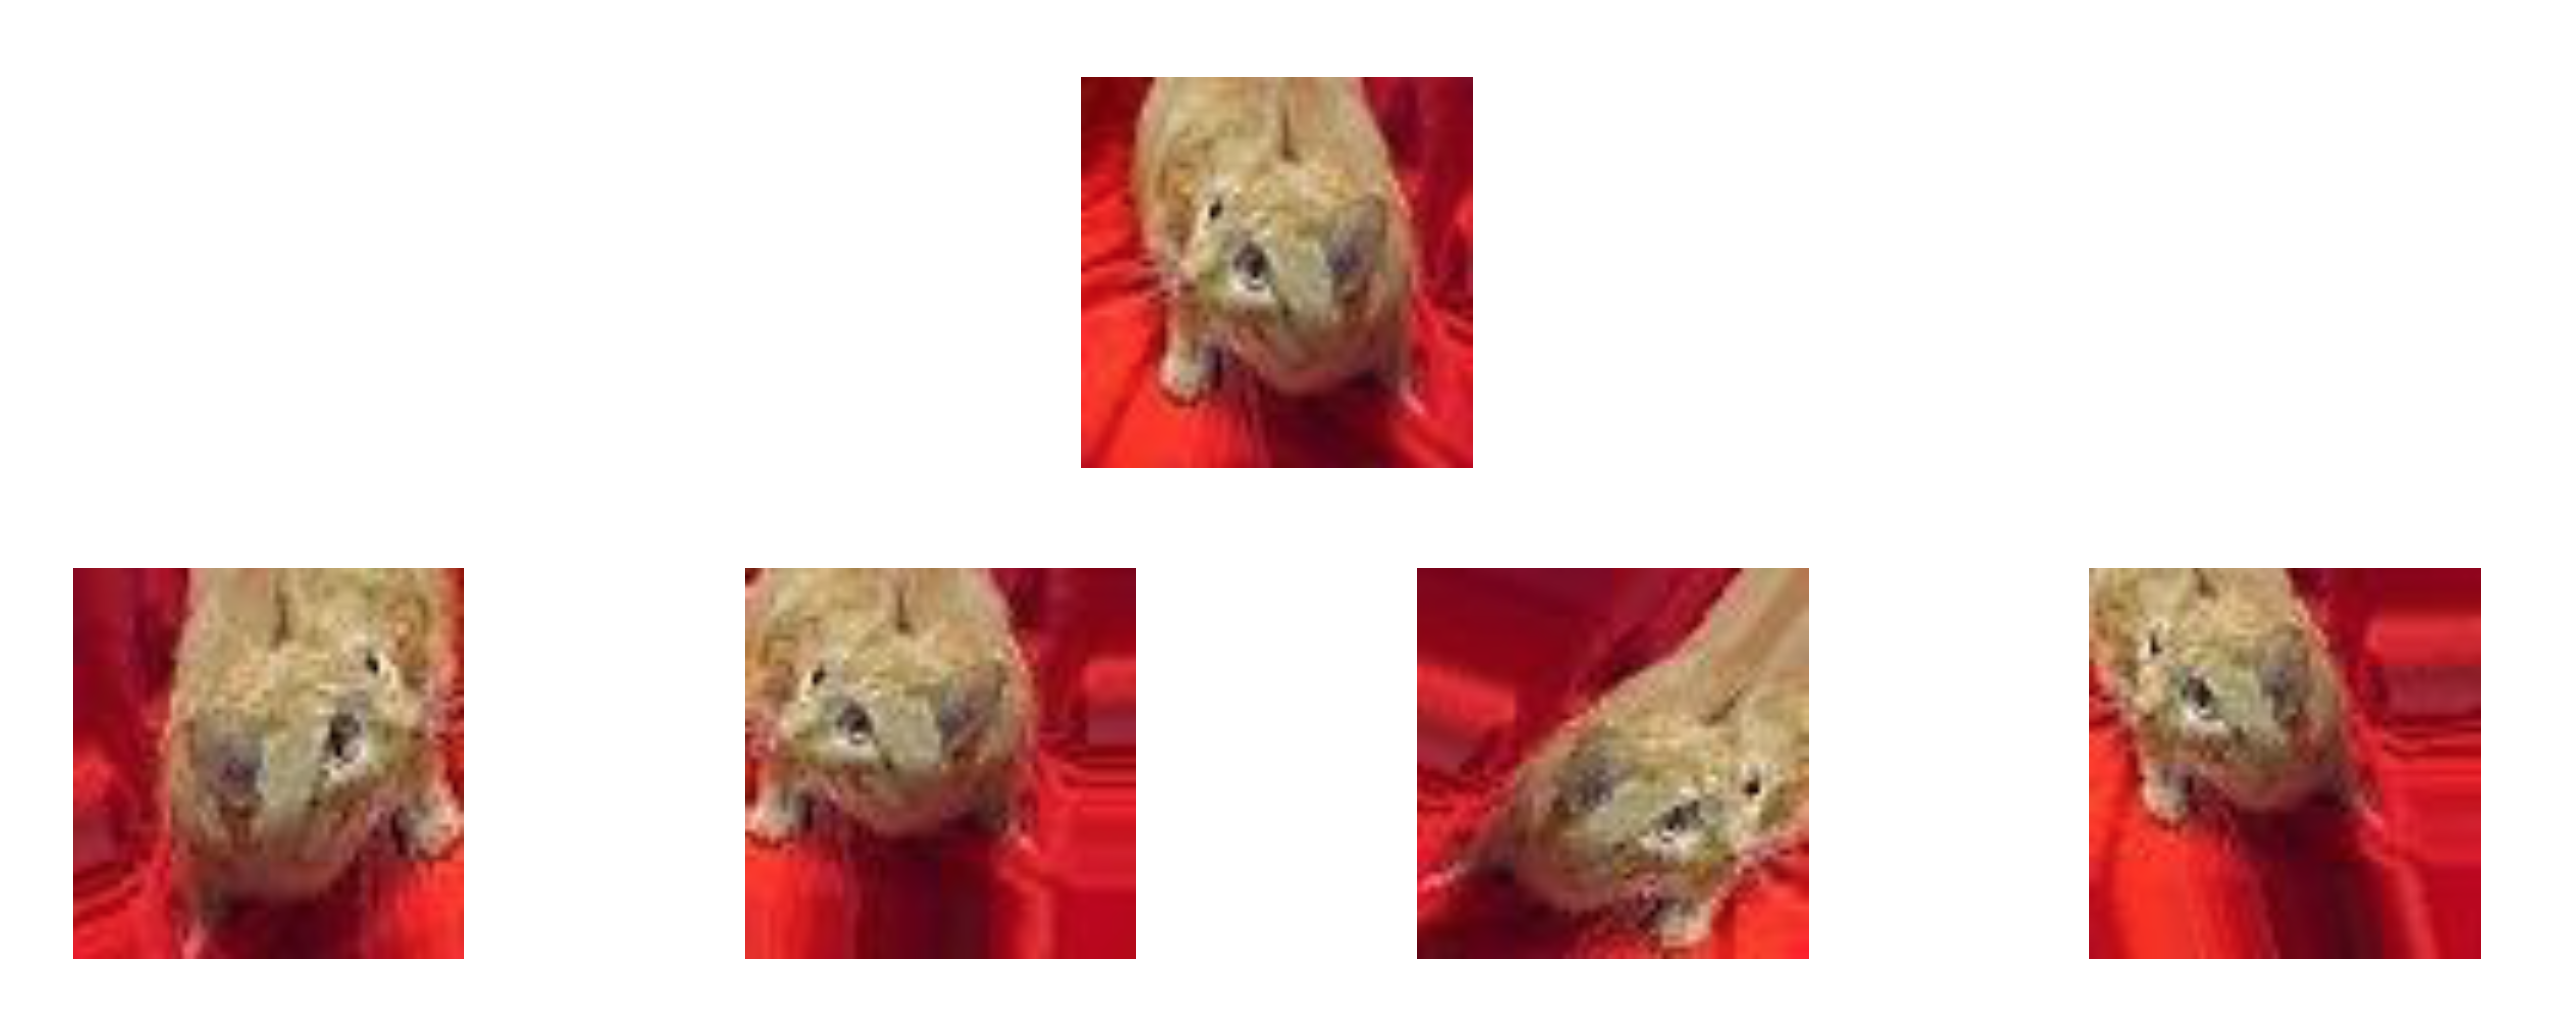
\includegraphics[scale=0.4]{res/catdogsaug.png}
\caption[Caption for LOF]{Obraz oryginalny oraz cztery obrazy wygenerowane na jego podstawie \label{catdogsimages}}
\end{figure} 

\subsubsection{Wyniki}
W~tabeli \ref{table:catdogs} przedstawione zostały wyniki dla sieci uruchamianej przy wykorzystaniu sztucznego powielania cech oraz~bez użycia tej techniki. Na~wykresach \ref{cd_1}, \ref{cd2}, \ref{cd3} przedstawione zostały kolejno skuteczności modelu na~danych testowych w~obu rozważanych przypadkach, skuteczność obliczana na~danych testowych oraz~uczących bez wykorzystania powielania danych, skuteczność obliczana na~danych testowych oraz~uczących przy wykorzystaniu techniki powielania danych.

\begin{table}
\centering
\begin{tabular}{|c|c|}
\hline
Skuteczność uzyskana przy wykorzystaniu sztucznego powielania danych & $72\% \pm 2\%$ \\
\hline 
Skuteczność uzyskana bez wykorzystania sztucznego powielania danych & $69\% \pm 2\%$ \\
\hline 
 \end{tabular}
 \caption{Porównanie wyników z~zastosowaniem metody sztucznego powielania danych} \label{table:catdogs}
\end{table}

\begin{figure}[ht!]
\centering
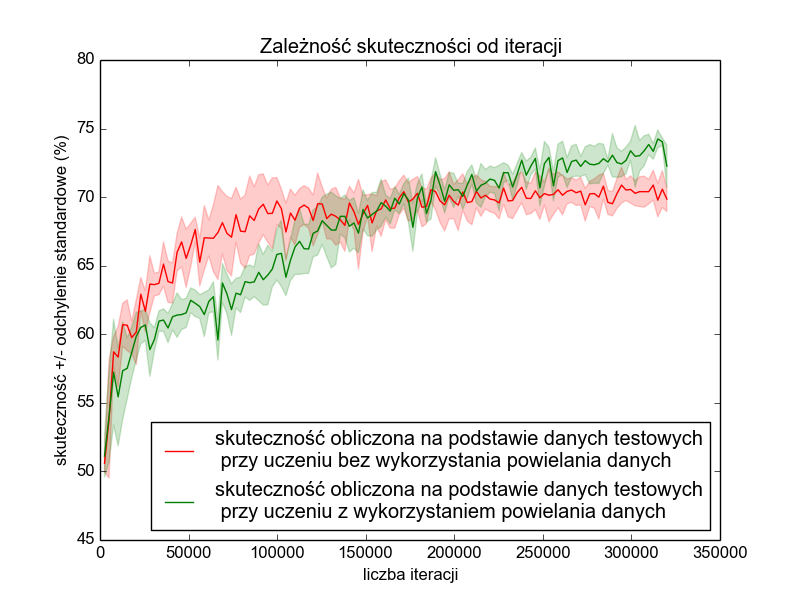
\includegraphics[scale=0.7]{res/comptest.png}
\caption[Caption for LOF]{Porównanie skuteczności w zależności od iteracji obliczana na danych testowych przy uczeniu przy wykorzystaniu powielania danych oraz bez użycia tej techniki\label{cd_1}}
\end{figure} 

\begin{figure}[ht!]
\centering
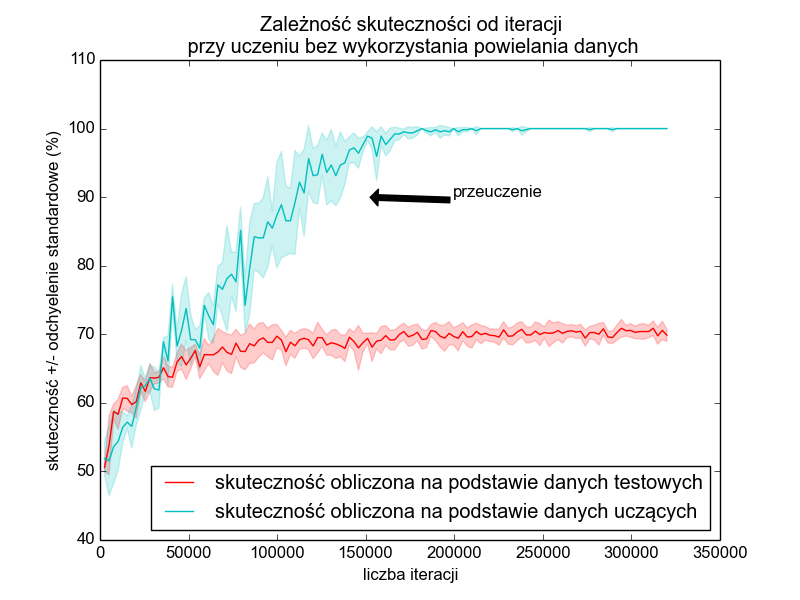
\includegraphics[scale=0.7]{res/testtrain_mulitply.png}
\caption[Caption for LOF]{Porównanie skuteczności w zależności od iteracji obliczana na danych testowych oraz uczących bez wykorzystania powielania danych\label{cd2}}
\end{figure} 

\begin{figure}[ht!]
\centering
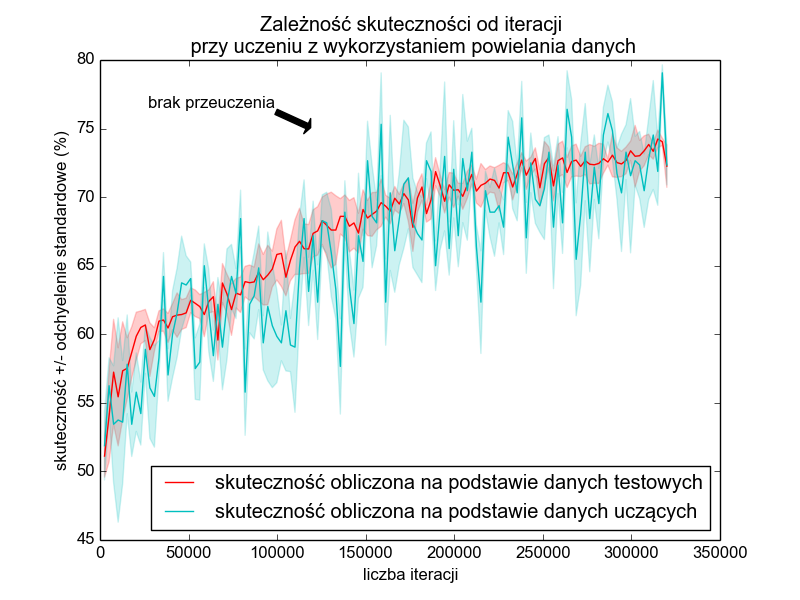
\includegraphics[scale=0.7]{res/testtrain_runtime.png}
\caption[Caption for LOF]{Porównanie skuteczności w zależności od iteracji obliczana na danych testowych oraz uczących z wykorzystania powielania danych\label{cd3}}
\end{figure} 

\subsubsection{Wnioski}
Sztuczne powiększanie zbioru danych, w~analizowanym przypadku nie przyniosło spektakularnej poprawy. Jest to jednak wciąż 2~\%, które~nie kosztuje zbyt wiele. Należy zwrócić uwagę też na~to, iż~w~rzeczywistym przypadku operacja ta może przynieść więcej korzyści pod~warunkiem odpowiedniego doboru jej parametrów, co nie zostało zrobione w~tym przypadku ze~względu na~ograniczone zasoby obliczeniowe. Spoglądając na~rysunek \ref{cd2} łatwo można zauważyć, że~w~przypadku, gdy podawaliśmy do~sieci niezmodyfikowane w~żaden sposób obrazy, szybko doszło do~przeuczenia. Skuteczność obliczana na~podstawie danych uczących osiągnęła 100\% i~sieć nie była w~stanie już więcej nauczyć się na~podstawie danych treningowych. W~przypadku gdy dane zostały sztucznie powielone, możemy zauważyć, na~rysunku \ref{cd3}, że~skuteczność dla zbioru testowego oraz~uczącego oscyluje na~podobnym poziomie w~kolejnych iteracjach. Prawdopodobnie, przeprowadzając uczenie dłużej tj. zwiększając liczbę iteracji, można byłoby spodziewać się, że~różnica w~wyniku przy obu podejściach mogłaby się powiększyć na~korzyść metody z~powielaniem danych, ponieważ~wciąż po~wyznaczonej liczbie iteracji nie doszło do~efektu przeuczenia.

\subsection{Walidacja krzyżowa}\label{cvChapter}
\subsubsection{Opis problemu}
W~tym podrozdziale autor starał się porównać system uczenia maszynowego działający przy zastosowaniu walidacji krzyżowej oraz~tradycyjnego podejścia w~którym zbiór danych jest dzielony na~zbiór uczący, testowy oraz~walidacyjny. Przeprowadzona została kolejno optymalizacja parametrów dla czterech algorytmów tj. maszyna wektorów nośnych, sztuczne sieci neuronowe, las drzew decyzyjnych oraz~pojedyncze drzewo decyzyjne. Sztuczna sieć neuronowa posiadała jedną warstwę ukrytą. Parametrami optymalizowanymi w~tym przypadku były: liczba neuronów w~warstwie ukrytej oraz~współczynnik uczenia. Dla lasu drzew decyzyjnych optymalizowana była liczba wykorzystanych drzew oraz~ich maksymalna głębokość, natomiast dla drzewa decyzyjnego optymalizowana była tylko maksymalna głębokość drzewa. W~przypadku maszyny wektorów nośnych dobierany był także tylko jeden parametr tj. współczynnik $C$ oraz~wykorzystany był kernel liniowy. W~każdym przypadku optymalizacja parametrów modelu została przeprowadzona za~pomocą metody walidacji krzyżowej oraz~wg tradycyjnego podejścia. Dla każdej pojedynczej optymalizacji następowało uczenie algorytmu 200 razy przed wyborem optymalnych wartości parametrów. W~przypadku wykorzystania walidacji krzyżowej dawało to $10*200$ dla przeprowadzenia optymalizacji. Algorytmy były testowane na~sztucznie wygenerowanych zbiorze zawierającym 7 atrybutów oraz~liczbę rekordów zawierającą się w~zbiorze $ \{200, 500, 1000, 1500, 2000\}.$ Następnie porównane zostały wyniki dla parametrów wyznaczonych wg obu metod dla wszystkich testowanych algorytmów. Należy zwrócić tutaj szczególną uwagę na~fakt, że~optymalizacja przy pomocy walidacji krzyżowej odbywa się na~poziomie doboru odpowiednich parametrów modelu. Po~określeniu parametrów modelu, bez względu na~metodę, którą do~tego wykorzystaliśmy, następuje uczenie oraz~walidacja finalnego modelu. W~przypadku obu podejść, przy uczeniu oraz~walidacji docelowego modelu, użyta zostaje dokładnie taka sama ilość danych. Porównanie użytej ilości danych w~obu przypadkach zostało przedstawione na~rysunku \ref{cvdata}. W~przypadku tradycyjnego podejścia zbiór danych został podzielony na~zbiór uczący stanowiący 60\% wszystkich danych, zbiór testowy stanowiący 20\% wszystkich danych oraz~zbiór walidujący - również 20\% wszystkich danych. W~przypadku walidacji krzyżowej, występowały tylko dwa zbiory tj. zbiór uczący oraz~zbiór walidujący stanowiące kolejno 80\% oraz~20\% wszystkich danych. W~celu uzyskania statystyki, obliczenia dla każdej metody dla konkretnej liczby rekordów powtórzone zostały 10 razy.

\begin{figure}[ht!]
\centering
\includegraphics[scale=0.6]{res/cvdata.png}
\caption[Caption for LOF]{Wykorzystanie danych w zleżności od zastosowanej metody doboru parametrów modelu\label{cvdata}}
\end{figure} 

\subsubsection{Stworzone rozwiązanie}
System stworzony w~celu porównania skuteczności modelu w~zależności od~użytej metody doboru parametrów modelu składał się komponentów takich jak~Main, Optimizer, oraz~Configuration. Pierwszy z~nich odpowiedzialny był za~rozpoczęcie wykonania całej procedury, uwzględniając także wygenerowanie odpowiednich danych. Komponenty nazwane Optimizer oraz~Configuration były kolejno odpowiedzialne za~optymalizację parametrów modelu wg wybranej metody oraz~ogólnej konfiguracji programu, gdzie można wybrać liczbę uruchomień optymalizacji czy~też liczbę rekordów dla których porównanie powinno zostać przeprowadzone. Przeprowadzanie wszystkich założonych obliczeń było bardzo czasochłonne ze~względu na~długość czasu przeprowadzania optymalizacji parametrów modelu, co trwa, w~zależność od~wybranych parametrów, od~kilkudziesięciu minut do~kilku godzin. Biorąc pod~uwagę liczbę możliwości dla tego przykładu, która~jest iloczynem liczby testowanych metod oraz~liczby rekordów dla których przeprowadzane zostały obliczenia, cały proces mógł trwać nawet ponad 40 godzin. W~celu optymalizacji pod~kątem czasu wykonywania programu, obliczenia zostały przeprowadzone z~wykorzystaniem wielowątkowości, co znacznie przyspiesza cały proces, zwłaszcza biorąc uwagę, że~maszyna wykorzystana dla tego zadania posiadała 12 wątków. 
 
\subsubsection{Wyniki}
Zbiorcze wyniki dla wszystkich testowanych wariantów zostały przedstawione w~tabeli \ref{table:cv}. Dla poszczególnych metod uczenia maszynowego, wyniki przedstawione zostały na~rysunkach \ref{cv_ann}, \ref{cv_svm}, \ref{cv_forest}, \ref{cv_tree} kolejno dla sztucznych sieci neuronowych, maszyny wektorów nośnych, lasu drzew decyzyjnych oraz~drzewa decyzyjnego.

% Please add the following required packages to your document preamble:
% \usepackage{multirow}
\begin{table}[]
\centering
\begin{tabular}{|l|l|l|l|l|l|}
\hline
liczba rekordów       & metoda   & ann & forest & svm & tree \\ \hline
\multirow{2}{*}{200}     & holdout    & $ (49,14 \pm 6,2) \% $ & $(45,86 \pm 9,18) \% $ & $(47,71 \pm 5,83) \% $ & $(37,57 \pm 8,48) \% $ \\ \cline{2-6} 
                         & cv         & $(52,14 \pm 5,16) \% $ & $(46,86 \pm 6,79) \% $ & $(48,71 \pm 6,27) \% $ & $(37,63 \pm 7,17) \% $ \\ \hline
\multirow{2}{*}{500}     & holdout    & $(54,4 \pm 5,68) \% $ & $(54,97 \pm 4,98) \% $ & $(50,51 \pm 3,99) \% $ & $(44,74 \pm 3,02) \% $ \\ \cline{2-6} 
                         & cv         & $(59,09 \pm 4,73) \% $ & $(60,34 \pm 3,55) \% $ & $(50,86 \pm 4,4) \% $ & $(45,2 \pm 1,72) \% $ \\ \hline
\multirow{2}{*}{1000}    & holdout    & $(64,11 \pm 3,69) \% $ & $(62,4 \pm 2,89) \% $ & $(56,6 \pm 5,2) \% $ & $(50,4 \pm 3,86) \% $ \\ \cline{2-6} 
                         & cv         & $(64,14 \pm 3,44) \% $ & $(67,51 \pm 4,03) \% $ & $(56,63 \pm 5,26) \% $ & $(49,77 \pm 3,43) \% $ \\\hline
\multirow{2}{*}{1500}    & holdout    &$ (69,24 \pm 2,72) \% $ & $(67,09 \pm 2,66) \% $ & $(58,36 \pm 3,8) \% $ & $(52,69 \pm 2,51) \% $ \\ \cline{2-6} 
                         & cv         & $(69,11 \pm 2,02) \% $ & $(70,97 \pm 1,39) \% $ & $(58,46 \pm 3,79) \% $ & $(52,5 \pm 3,13) \% $ \\ \hline
\multirow{2}{*}{2000}    & holdout    & $(67,74 \pm 4,52) \% $ & $(69,57 \pm 3,5) \% $ & $(58,34 \pm 6,08) \% $ & $(56,44 \pm 3,92) \% $ \\ \cline{2-6} 
                                          & cv         & $(67,74 \pm 4,49) \% $ & $(72,37 \pm 3,01) \% $ & $(58,24 \pm 6,14) \% $ & $(56,71 \pm 3,69) \% $ \\ \hline
                                                                                    
\multicolumn{2}{|l|}{średnia poprawa}   &  $1,52 \%$    &  $3,63 \%$      &  $0,27 \%$   &  $-0,01 \%$   \\ \hline

\end{tabular}
\caption{Skuteczność modelu dla danych walidacyjnych w zależności od testowanego algorytmu uczenia maszynowego oraz wykorzystanej metody optymalizacji parametrów} \label{table:cv}
\end{table}

\newcommand{\cvsize}{1}


\begin{figure}
\centering
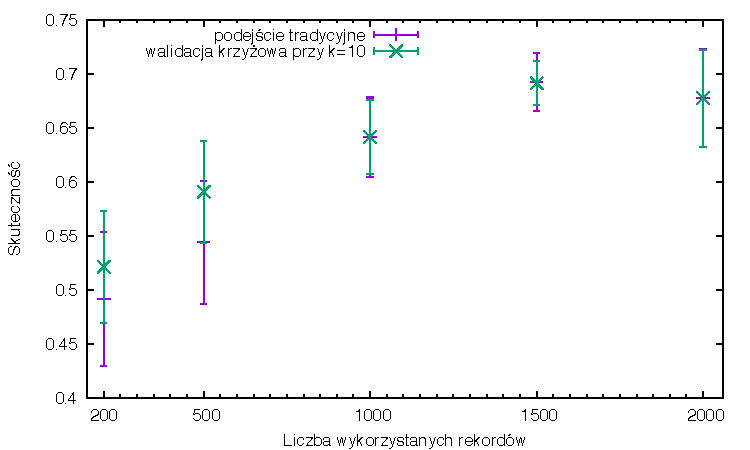
\includegraphics[scale=\cvsize]{res/cv_ann.pdf}
\caption[Caption for LOF]{Porównanie skuteczności modelu przy optymalizacji parametrów przy użyciu walidacji krzyżowej oraz tradycyjnego podejścia dla sztucznych sieci neuronowych\label{cv_ann}}
\end{figure}

\begin{figure}
\centering
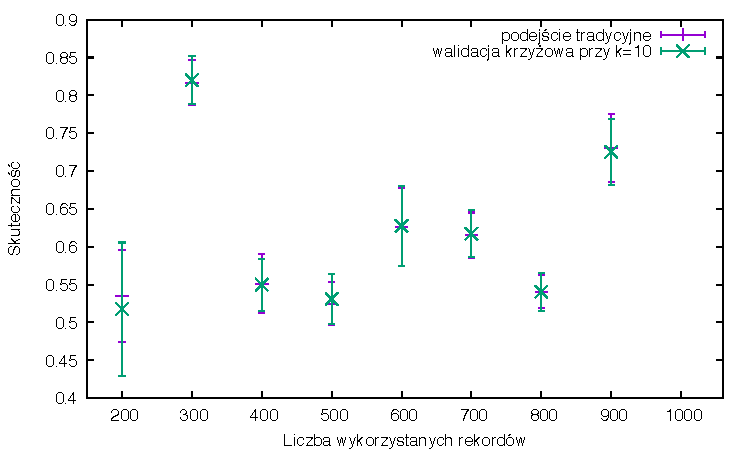
\includegraphics[scale=\cvsize]{res/cv_svm.pdf}
\caption[Caption for LOF]{Porównanie skuteczności modelu przy optymalizacji parametrów przy użyciu walidacji krzyżowej oraz tradycyjnego podejścia dla maszyny wektorów wspierających\label{cv_svm}}
\end{figure}

\begin{figure}
\centering
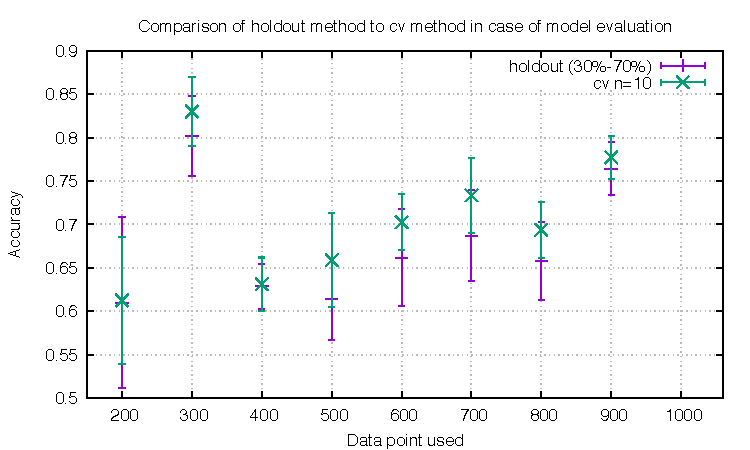
\includegraphics[scale=\cvsize]{res/cv_forest.pdf}
\caption[Caption for LOF]{Porównanie skuteczności modelu przy optymalizacji parametrów przy użyciu walidacji krzyżowej oraz tradycyjnego podejścia dla lasu drzew decyzyjnych\label{cv_forest}}
\end{figure}

\begin{figure}
\centering
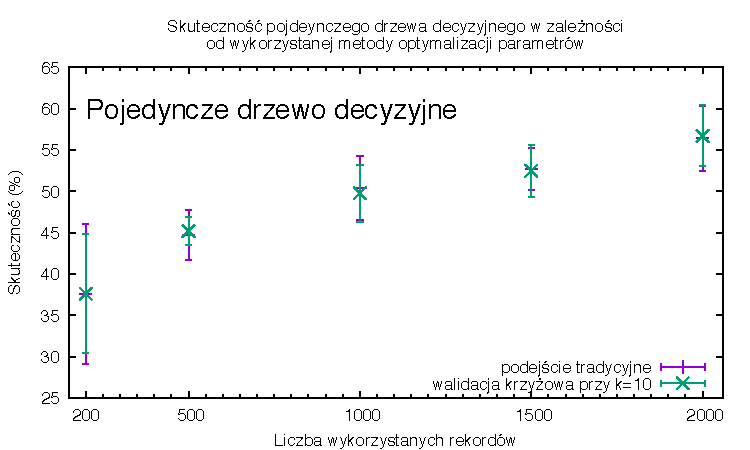
\includegraphics[scale=\cvsize]{res/cv_tree.pdf}
\caption[Caption for LOF]{Porównanie skuteczności modelu przy optymalizacji parametrów przy użyciu walidacji krzyżowej oraz tradycyjnego podejścia dla drzewa decyzyjnego\label{cv_tree}}
\end{figure}
  


\subsubsection{Wnioski}
Analizując wyniki można stwierdzić, że~poprawa skuteczności klasyfikacji przy użyciu walidacji krzyżowej w~celu wyboru parametrów modelu zależy od~stosowanego algorytmu, a~także od~tego jak~duża liczba rekordów wykorzystana zostaje przy uczeniu algorytmu. Zdecydowanie im więcej rekordów, tym mniejsza poprawa skuteczności. Wynika to z~faktu, iż~powyżej pewnej ilości danych algorytm nie jest w~stanie nauczyć się więcej. Spoglądając na~wykres \ref{cv_ann} możemy zauważyć, że~w~przypadku sieci neuronowych, przy niższej ilości danych, tj. 200 oraz~500 rekordów, poprawa wynosi aż kilka procent, co jest bardzo zadowalającym wynikiem. W~przypadku większej liczby rekordów wynik jest porównywalny bez względu na~wykorzystaną metodę optymalizacji. W~przypadku drzewa decyzyjnego oraz~maszyny wektorów wspierających wartość skuteczności nie różni się na~tyle, aby~mówić o~jakiejkolwiek zmianie bez względu na~użytą metodę doboru parametrów, co może wynikać z~faktu, iż~w~przypadku obu tych metod tylko jeden parametr był optymalizowany (w przypadku sieci neuronowyh oraz~lasu drzew decyzyjnych były optymalizowane 2 parametry). Wpływ optymalizacji na~skuteczność jest mniejszy w~takim przypadku. Zwiększyć można byłoby go poprzez~rozszerzenie zakresu optymalizacji.

\subsection{Ekstrakcja cech przy użyciu metod matematycznych}

\subsubsection{Opis problemu}
Metodę wykorzystaną w~celu ekstrakcji cech w~ramach metod matematycznych była liniowa analiza dyskryminacyjna. Przetestowane zostały cztery algorytmy uczenia maszynowego tj. maszyna wektorów nośnych, sztuczne sieci neuronowe, las drzew decyzyjnych oraz~pojedyncze drzewo decyzyjne. Wykorzystanym zbiorem danych był zbiór o~nazwie \textit{iris} dostępny w~bibliotece Scikit-Learn\footnote{\url{http://scikit-learn.org/stable/auto_examples/datasets/plot_iris_dataset.html}}. Posiada on 4 atrybuty, które~mówią o~rozmiarach irysów 3 różnych gatunków, a~więc, co za~tym idzie, cały zbiór podzielony jest na~3 klasy. Każdy rekord zbioru reprezentuje kwiat. Zbiór zawiera 150 rekordów, po~50 dla każdej gatunku. Zbiór ten był wprowadzony przez~brytyjskiego statystyka oraz~biologa Ronalda Fishera, którego~rola była znacząca w~rozwoju statystyki. Eksperyment polegał na~kolejno:
\begin{itemize}

\item przeprowadzeniu optymalizacji parametrów modeli dla poszczególnych metod,
\item uczeniu oraz testowaniu systemu.

\end{itemize}

Powyższe kroki wykonane zostały w~zależności od~liczby rekordów oraz~liczby atrybutów zbioru. Liczba rekordów dla których przeprowadzone zostały testy mieściła się w~zbiorze $ \{10, 20, 30, 40, 50, 100\} $. Obliczenia przeprowadzone zostały dla liczby atrybutów początkowo wynoszącej 4, 2 oraz~1. Celem było określenie czy, oraz~na~ile, ekstrakcja cech może pomóc w~otrzymaniu wyższej skuteczności przy uczeniu maszynowym. Wszystkie obliczenia wykonane zostały w~każdym przypadku 10 razy w~celu uzyskania odpowiedniej statystyki wyników.

\subsubsection{Stworzone rozwiązanie}
Stworzony system składał się z~komponentów takich jak~Main, Optimizer oraz~Configuration. Podobnie jak~w~eksperymencie opisanym w~podrozdziale \ref{cvChapter} były odpowiedzialne kolejno za~zadania uruchomienia głównego programu, optymalizacji parametrów modelu oraz~konfigurację. Dodatkowo, w~komponencie Main, znajduję się logika programu odpowiedzialna za~redukcję wymiarowości zbioru danych. Także i~w tym przypadku wykonywanie całej procedury dla różnych przypadków trwało dość długo tj. od~kilku do~kilkunastu godzin, co stanowiło motywację do~wykorzystania wielowątkowości.

\subsubsection{Wyniki}
Zbiorcze wyniki dla różnej ilości wykorzystanych danych zostały przedstawione w~tabeli \ref{table:fxTable} oraz~na~rysunku \ref{extractionSummary}. Dodatkowo, na~rysunku \ref{showMeIris} przedstawiony został zbiór danych \textit{iris} pod~redukcji do~dwóch wymiarów oraz~do~jednego wymiaru.


\begin{figure}[ht!]
\centering
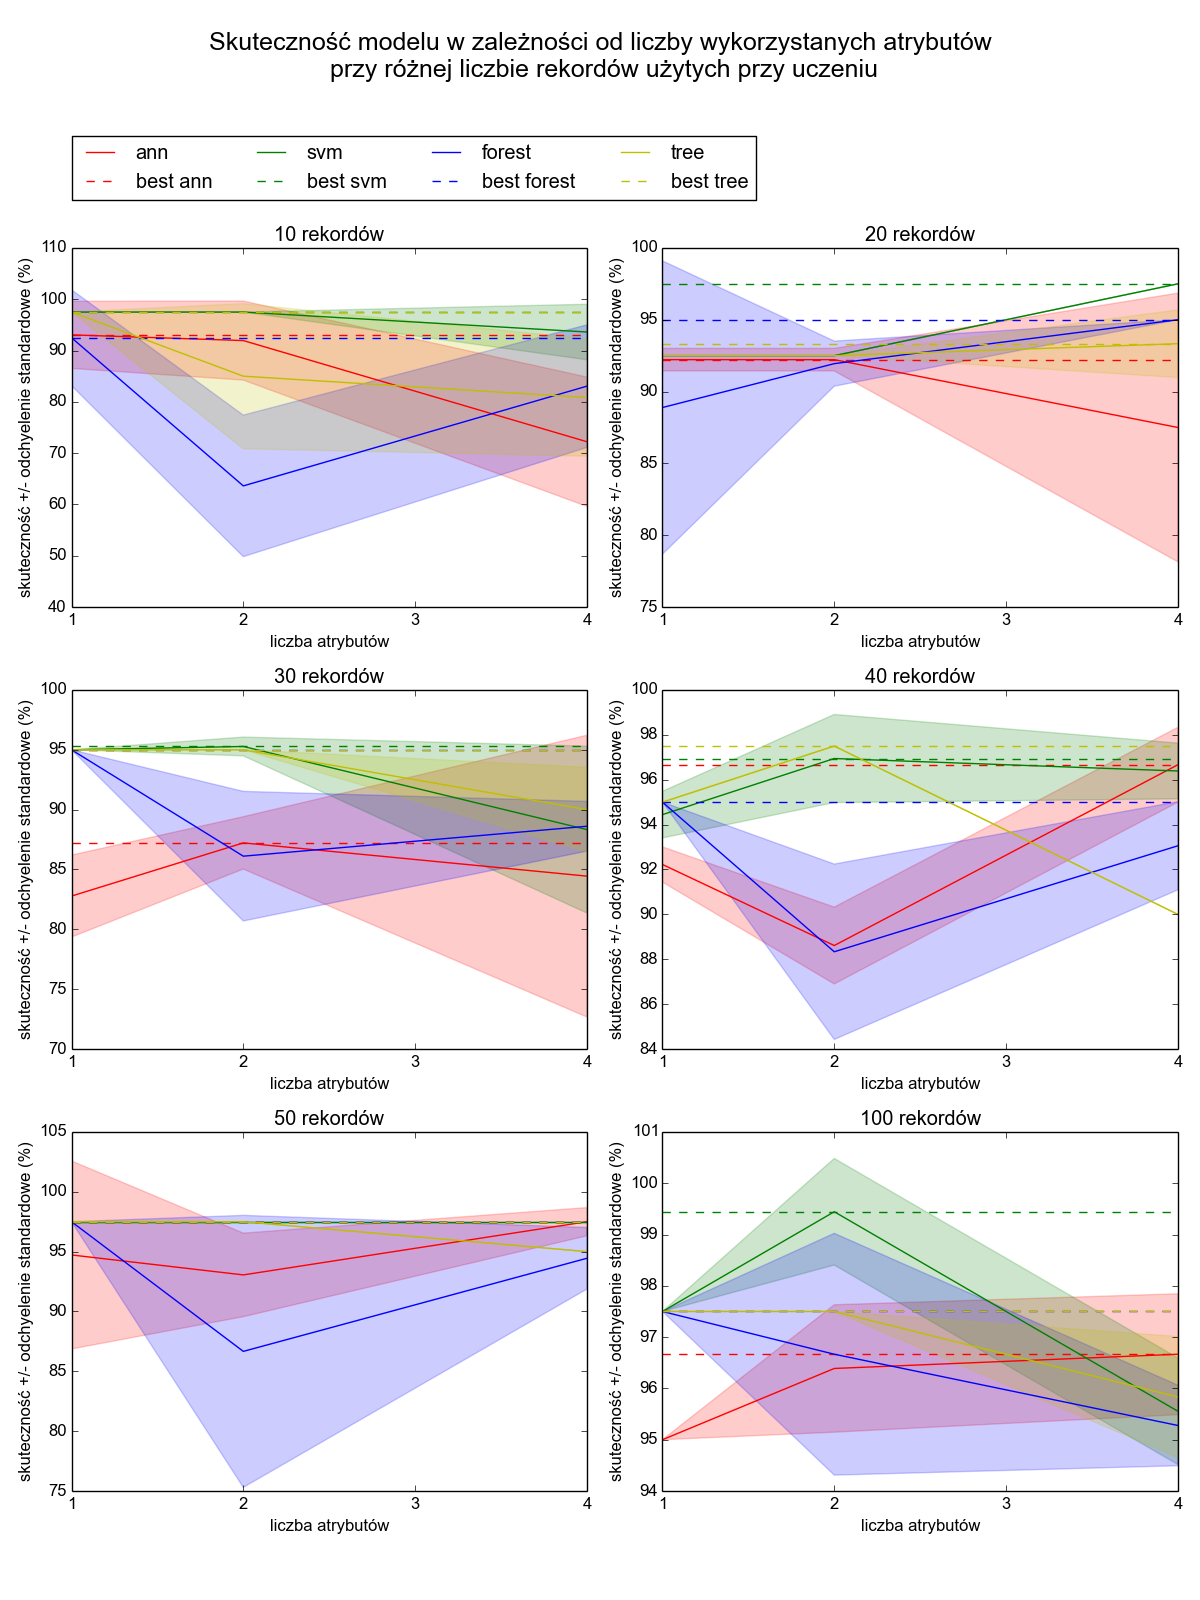
\includegraphics[scale=0.45]{res/extractionSummary.png}
\caption[Caption for LOF]{Porwóananie skuteczności modelu dla różnych algorytmów w zależności od liczby atrybutów oraz ilości wykorzystanych do uczenia danych\label{extractionSummary}}
\end{figure} 

\begin{figure}[ht!]
\centering
\includegraphics[scale=0.45]{res/showMeIris.png}
\caption[Caption for LOF]{Zbiór danych \textit{iris} po przeprowadzeniu ekstrakcji cech\label{showMeIris}}
\end{figure} 

% Please add the following required packages to your document preamble:
% \usepackage{multirow}
\begin{table}[]
\tiny
\centering
\begin{tabular}{|c|c|c|c|c|}
\hline
Liczba rekordów       & Metoda                  & Liczba atrybutów & Skuteczność & Poprawa \\ \hline
\multirow{12}{*}{10}  & \multirow{3}{*}{ann}    & 1                & $ (93,06  \pm  6,54) \% $ & \multirow{3}{*}{$20,84\%$} \\ \cline{3-4} 
                      &                         & 2                & $ (91,94 \pm 7,71) \% $   & \\ \cline{3-4} 
                      &                         & 4                & $ (72,22 \pm 12,61) \% $  & \\ \cline{2-5} 
                      & \multirow{3}{*}{svm}    & 1                & $ (97,5 \pm 0) \% $        & \multirow{3}{*}{$3,89 \%$} \\ \cline{3-4} 
                      &                         & 2                & $ (97,5 \pm 0) \% $       &\\ \cline{3-4} 
                      &                         & 4                & $ (93,61 \pm 5,41) \% $   &\\ \cline{2-5} 
                      & \multirow{3}{*}{forest} & 1                & $ (92,5 \pm 9,35) \% $    & \multirow{3}{*}{$9,44\%$} \\ \cline{3-4} 
                      &                         & 2                & $ (63,61 \pm 13,8) \% $   &\\ \cline{3-4} 
                      &                         & 4                & $ (83,06 \pm 11,95) \% $ & \\ \cline{2-5} 
                      & \multirow{3}{*}{tree}   & 1                & $ (97,5 \pm 0) \% $       & \multirow{3}{*}{$16,67\%$} \\ \cline{3-4} 
                      &                         & 2                & $ (85 \pm  14,14) \% $    & \\ \cline{3-4} 
                      &                         & 4                & $ (80,83 \pm 11,43) \% $  &\\ \hline
\multirow{12}{*}{20}  & \multirow{3}{*}{ann}    & 1                & $ (92,22 \pm 0,79) \% $   & \multirow{3}{*}{$4,72\%$} \\ \cline{3-4} 
                      &                         & 2                & $ (92,22 \pm 0,79) \% $   &\\ \cline{3-4} 
                      &                         & 4                & $ (87,5 \pm 9,35) \% $    &\\ \cline{2-5} 
                      & \multirow{3}{*}{svm}    & 1                & $ (92,5 \pm 0) \% $       & \multirow{3}{*}{$-5 \%$} \\ \cline{3-4} 
                      &                         & 2                & $ (92,5 \pm 0) \% $       &\\ \cline{3-4} 
                      &                         & 4                & $ (97,5 \pm 0) \% $       &\\ \cline{2-5} 
                      & \multirow{3}{*}{forest} & 1                & $ (88,89 \pm 10,21) \% $  & \multirow{3}{*}{$-3,06 \%$} \\ \cline{3-4} 
                      &                         & 2                & $ (91,94 \pm 1,57) \% $  & \\ \cline{3-4} 
                      &                         & 4                & $ (95 \pm 0) \% $         &\\ \cline{2-5} 
                      & \multirow{3}{*}{tree}   & 1                & $ (92,5 \pm 0) \% $       & \multirow{3}{*}{$-0,83 \%$} \\ \cline{3-4} 
                      &                         & 2                & $ (92,5 \pm 0) \% $       &\\ \cline{3-4} 
                      &                         & 4                & $ (93,33 \pm 2,36) \% $   &\\ \hline
\multirow{12}{*}{30}  & \multirow{3}{*}{ann}    & 1                & $ (82,78 \pm 3,42) \% $   & \multirow{3}{*}{$2,78\%$} \\ \cline{3-4} 
                      &                         & 2                & $ (87,22 \pm 2,19) \% $  & \\ \cline{3-4} 
                      &                         & 4                & $ (84,44 \pm 11,77) \% $  &\\ \cline{2-5} 
                      & \multirow{3}{*}{svm}    & 1                & $ (95 \pm 0) \% $        & \multirow{3}{*}{$6,95\%$} \\ \cline{3-4} 
                      &                         & 2                & $ (95,28 \pm 0,79) \% $   &\\ \cline{3-4} 
                      &                         & 4                & $ (88,33 \pm 6,97) \% $   &\\ \cline{2-5} 
                      & \multirow{3}{*}{forest} & 1                & $ (95 \pm 0) \%  $        & \multirow{3}{*}{$6,39\%$} \\ \cline{3-4} 
                      &                         & 2                & $ (86,11 \pm 5,41) \% $   &\\ \cline{3-4} 
                      &                         & 4                & $ (88,61 \pm 2,08) \% $  & \\ \cline{2-5} 
                      & \multirow{3}{*}{tree}   & 1                & $ (95 \pm 0) \%  $       & \multirow{3}{*}{$5\%$} \\ \cline{3-4} 
                      &                         & 2                & $ (95 \pm 0) \%  $       &\\ \cline{3-4} 
                      &                         & 4                & $ (90 \pm  3,54) \% $     & \\ \hline
\multirow{12}{*}{40}  & \multirow{3}{*}{ann}    & 1                & $ (92,22 \pm 0,79) \% $   & \multirow{3}{*}{$-4,55  \%$} \\ \cline{3-4} 
                      &                         & 2                & $ (88,61 \pm 1,71) \% $   &\\ \cline{3-4} 
                      &                         & 4                & $ (96,67 \pm 1,67) \% $  & \\ \cline{2-5} 
                      & \multirow{3}{*}{svm}    & 1                & $ (94,44 \pm 1,04) \% $   & \multirow{3}{*}{$0,55$\%} \\ \cline{3-4} 
                      &                         & 2                & $ (96,94 \pm 1,96) \% $  & \\ \cline{3-4} 
                      &                         & 4                & $ (96,39 \pm 1,24) \% $   &\\ \cline{2-5} 
                      & \multirow{3}{*}{forest} & 1                & $ (95 \pm 0) \% $        & \multirow{3}{*}{$1,94$\%} \\ \cline{3-4} 
                      &                         & 2                & $ (88,33 \pm 3,91) \% $   &\\ \cline{3-4} 
                      &                         & 4                & $ (93,06 \pm 1,96) \% $   &\\ \cline{2-5} 
                      & \multirow{3}{*}{tree}   & 1                & $ (95 \pm 0) \% $         & \multirow{3}{*}{$7,5\%$} \\ \cline{3-4} 
                      &                         & 2                & $ (97,5 \pm 0) \% $      &\\ \cline{3-4} 
                      &                         & 4                & $ (90 \pm 0) \%   $     & \\ \hline
\multirow{12}{*}{50}  & \multirow{3}{*}{ann}    & 1                & $ (94,72 \pm 7,86) \% $   & \multirow{3}{*}{$-2,78 \%$} \\ \cline{3-4} 
                      &                         & 2                & $ (93,06 \pm 3,49) \% $  & \\ \cline{3-4} 
                      &                         & 4                & $ (97,5 \pm 1,18) \% $    &\\ \cline{2-5} 
                      & \multirow{3}{*}{svm}    & 1                & $ (97,5 \pm 0) \% $       & \multirow{3}{*}{$0 \%$} \\ \cline{3-4} 
                      &                         & 2                & $ (97,5 \pm 0) \% $     &  \\ \cline{3-4} 
                      &                         & 4                & $ (97,5 \pm 0) \% $       & \\ \cline{2-5} 
                      & \multirow{3}{*}{forest} & 1                & $ (97,5 \pm 0) \% $       & \multirow{3}{*}{$3.06\%$} \\ \cline{3-4} 
                      &                         & 2                & $ (86,67 \pm 11,37) \% $ & \\ \cline{3-4} 
                      &                         & 4                & $ (94,44 \pm 2,58) \% $   &\\ \cline{2-5} 
                      & \multirow{3}{*}{tree}   & 1                & $ (97,5 \pm 0) \% $       & \multirow{3}{*}{$2.5\%$} \\ \cline{3-4} 
                      &                         & 2                & $ (97,5 \pm 0) \% $      & \\ \cline{3-4} 
                      &                         & 4                & $ (95 \pm 0) \%   $      &\\ \hline
\multirow{12}{*}{100} & \multirow{3}{*}{ann}    & 1                & $ (95 \pm 0) \%   $      & \multirow{3}{*}{$-1,67 \%$} \\ \cline{3-4} 
                      &                         & 2                & $ (96,39 \pm 1,24) \% $   &\\ \cline{3-4} 
                      &                         & 4                & $ (96,67 \pm 1,18) \% $  & \\ \cline{2-5} 
                      & \multirow{3}{*}{svm}    & 1                & $ (97,5 \pm 0) \% $       & \multirow{3}{*}{$3,88\%$} \\ \cline{3-4} 
                      &                         & 2                & $ (99,44 \pm 1,04) \% $  & \\ \cline{3-4} 
                      &                         & 4                & $ (95,56 \pm 1,04) \% $  & \\ \cline{2-5} 
                      & \multirow{3}{*}{forest} & 1                & $ (97,5 \pm 0) \% $       & \multirow{3}{*}{$2,22\%$} \\ \cline{3-4} 
                      &                         & 2                & $ (96,67 \pm 2,36) \% $   &\\ \cline{3-4} 
                      &                         & 4                & $ (95,28 \pm 0,79) \% $  & \\ \cline{2-5} 
                      & \multirow{3}{*}{tree}   & 1                & $ (97,5 \pm 0) \% $       & \multirow{3}{*}{$1,67\%$} \\ \cline{3-4} 
                      &                         & 2                & $ (97,5 \pm 0) \% $       &\\ \cline{3-4} 
                      &                         & 4                & $ (95,83 \pm 1,18) \% $   &\\ \hline
\end{tabular}
\caption{Zestawienie skuteczności przy wykorzystaniu ekstrakcji cech przy użyciu różnej liczby rekordów, różne liczby atrybutów w zależności od wybranej metody}
\label{table:fxTable}

\end{table}

\subsubsection{Wnioski}
Analizując jako pierwszy wykres na~rysunku \ref{showMeIris}, można zauważyć, że~dane ze~zbioru \textit{iris} są prawie separowalne liniowo. Stwarza to możliwość efektywnego wykorzystania metody LDA w~celu ekstrakcji cech. Trzeba jednak pamiętać, że~tego typu zbiory raczej nie są zbyt często spotykane w~rzeczywistości. Wykres przedstawiający opracowywane dane w~jednym wymiarze pokazuje, że~transformacja do~takiej przestrzeni nie stanowi wciąż problemu jeśli chodzi o~realizację zadania klasyfikacji w~tym przypadku. Posiadanie danych o~mniejszej ilości atrybutów pozwala użyć prostszych modeli, co z~kolei przeciwdziała przeuczeniu, które~jest znacznym problemem w~przypadku niskiej ilości danych. W~przypadku posiadania tylko 10 rekordów w~celu przeprowadzenia uczenia, można zauważyć jak~bardzo pomocna okazuje się tutaj ekstrakcja cech. Poprawa skuteczności została odnotowana dla wszystkich metod i~to bardzo w~znacznym stopniu w~przypadku algorytmu drzewa decyzyjnego oraz~sztucznych sieci neuronowych, bo~aż $16,67 \%$ w~pierwszym oraz~$20,84 \%$ przypadku drugim (patrz tabela \ref{table:fxTable}). Dla lasu drzew decyzyjnych oraz~maszyny wektorów wspierających poprawa wynosiła kolejno $9,44 \%$ oraz~$3,89 \%$, co wciąż jest zadowalającym wynikiem.  Należy jednak zwrócić jednak na~odchylenie standardowe. Jego wysoka wartość oznacza duże fluktuacje. Z~reguły im mniej danych było wykorzystywanych, tym większa wartość odchylenia standardowego była odnotowywana. Jest to naturalne zjawisko. Im mniej danych, tym wynik jest bardziej przypadkowy ze~względu na~fakt, iż~dane uczące są losowo wybierane z~całego zbioru. W~niektórych przypadkach można też zauważyć bardzo niewielką zmianą albo~też nawet całkowity jej brak jeśli chodzi o~wynik oraz~odchylenie standardowe (np. SVM dla 50 rekordów). Jest to również pozytywne zjawisko. Korzystając z~danych o~mniejszej liczbie wymiarów udało się osiągnąć ten sam efekt, co oznacza, że~mniej obliczeń zostało przeprowadzonych, a~skuteczność oraz~odchylenie standardowe pozostały na~podobnym poziomie. Przy większej ilości danych, poprawa skuteczności nie zawsze występowała, ale~wciąż w~większości przypadków wyniki uzyskiwane po~przeprowadzeniu ekstrakcji były lepsze (poprawa została odnotowana w~13 na~20 pozostałych przypadków). Podsumowując, ekstrakcja cech stanowi bardzo dobry sposób na~optymalizację uczenia maszynowego pod~kątem ilości danych, lecz wydaje się, że~nie może być bardzo często stosowana ze~względu na~wymóg liniowej separowalność danych. Istnieją jednakże algorytmy, które~są w~stanie przeprowadzić ekstrakcję danych, które~nie są separowalne liniowo. Sama sieć neuronowa może zostać wykorzystana w~celu nielinowej ekstrakcji cech.  Podejście to zostało opisane w~pracy \cite{bishop1995neural} (strona 314).

\subsection{Ekstrakcja cech przy użyciu ,,wiedzy''}
\subsubsection{Opis problemu}
W~niniejszym podrozdziale rozważanym zagadnieniem była ekstrakcja cech przy użyciu ,,wiedzy'', która~polega na~transformacji danych do~przestrzeni o~mniejszej wymiarowości przy wykorzystaniu wiedzy, którą posiadamy na~temat naszych danych. Pomysł na~ten eksperyment został zaczerpnięty z~pracy~\cite{higgs1}. Wykorzystane zostały także dane opisane w~artykule, które~są danymi symulowanymi mającymi posłużyć jako podstawa dla stworzenia modelu, który~jest w~stanie odróżnić tło od~sygnału przy czym w~tym przypadku sygnałem jest bozon Higgsa, którego~istnienie zostało potwierdzone w~2013 roku. 
Badania dotyczące fizyki cząstek przeprowadzane sa  w~Europejskim Ośrodku Badań Jądrowych CERN w~pobliżu Genewy. Najbardziej spektakularnym narzędziem do~tego wykorzystywanym jest Wielki Zderzacz Hadronów (\textit{Large Hadron Collider}, LHC), który~jest największym na~świecie akceleratorem cząstek na~świecie. W~celu izolacji sygnału od~tła, w~przypadku danych z~odpowiednich detektorów cząstek, szeroko wykorzystywane jest uczenie maszynowe. Artykuł opisuje wykorzystanie głębokich sieci neuronowych dla problemu wyodrębnienia cząstki Higgsa. Udostępnione dane zawierają 11 milionów rekordów dla których określonych jest 21 cech fizycznych tzw. niskiego poziomu. Każdy rekord opisany jest także za~pomocą 7 atrybutów wysokiego poziomu, które~obliczone zostały na~podstawie cech niskiego poziomu. Celem obliczeń było pokazanie, że~poniżej pewnej ilości danych, użycie niskiego poziomu daje gorsze wyniki niż wykorzystanie cech wysokiego poziomu. Ekstrakcja cech przy użyciu ,,wiedzy'' można więc traktować jako optymalizację pod~kątem niskiej ilości danych. Obok głębokiej sieci neuronowej, wykorzystane zostały algorytmy takie jak~tradycyjne sieć neuronowa, las drzew decyzyjnych oraz~pojedyncze drzewo decyzyjne. Dla wszystkich wymienionych tradycyjnych algorytmów uczenia maszynowego przeprowadzona została optymalizacja parametrów. W~przypadku głębokiej sieci neuronowej nie miało to miejsca ze~względu na~bardzo długi czas uczenia. W~przypadku wszystkich metod obliczenia przeprowadzone zostały dla cech wysokiego oraz~niskiego poziomu, a~także dla różnej ilości danych, które~były fragmentami całego udostępnionego zbioru. Rozważone zostały ułamki $a$ całego zbioru przy czym $a\in\{0,001; 0,005; 0,01; 0,05; 0,1; 0,2; 0,3; 0,4; 0,5\}$. 

\subsubsection{Stworzone rozwiązanie}
Stworzony system składał się z~trzech elementów z~których można wyróżnić: HiggsModel, Optimizer oraz~Configuration. Były odpowiedzialne kolejno za~tworzenie głębokie sieci neuronowej (oparty na~pracy \cite{higgs2}), optymalizację parametrów dla poszczególnych algorytmów oraz~konfiguracji programu. W~przypadku głębokiej sieci neuronowej, wykorzystana została sieć posiadająca 6 warstw ukrytych po~500 neuronów w~każdej. Podobnie jak~w~przypadków poprzednich obliczeń, autor skorzystał z~dobrodziejstw wielowątkowości w~celu ich przyspieszenia.


\subsubsection{Wyniki}
Na~rysunkach \ref{higgsall1} oraz~\ref{higgsall2} przedstawione została krzywa ROC dla $a\in\{0,001; 0,005; 0,01; 0,05; 0,1\}$  oraz~dla $a\in\{0,2; 0,3; 0,4; 0,5\}$. AUC ROC dla wszystkich testowanych kombinacji zostało przedstawione w~tabeli \ref{table:higgstable} oraz~przedstawione na~rysunku \ref{higgssummary}.


% Please add the following required packages to your document preamble:
% \usepackage{multirow}
\begin{table}[]
\centering
\begin{tabular}{|c|c|c|c|c|c|}
\hline
\multirow{2}{*}{a}                      &  \multirow{2}{*}{wykorzystane cechy} & \multicolumn{4}{c|}{AUC ROC} \\ \cline{3-6}

 &       & tree & forest & ann & dnn \\ \hline

\multirow{2}{*}{0,001} & niskiego poziomu   & $ 0,6 $ & $ 0,62 $ & $ 0,62 $ &$ 0,62 $ \\ \cline{2-6} 
                       & wysokiego poziomu & $ 0,71 $ & $ 0,77 $ & $ 0,66 $ &$ 0,72 $ \\ \hline 
                       
\multirow{2}{*}{0,005} & niskiego poziomu  & $ 0,63 $ & $ 0,63 $ & $ 0,63 $ &$ 0,67 $ \\ \cline{2-6} 
                       & wysokiego poziomu & $ 0,74 $ & $ 0,75 $ & $ 0,69 $ &$ 0,77 $ \\ \hline
                       
\multirow{2}{*}{0,01}  & niskiego poziomu  & $ 0,64 $ & $ 0,64 $ & $ 0,63 $ &$ 0,7 $ \\ \cline{2-6} 
                       & wysokiego poziomu & $ 0,74 $ & $ 0,75 $ & $ 0,7 $ &$ 0,77 $ \\ \hline
                       
\multirow{2}{*}{0,05}  & niskiego poziomu  & $ 0,66 $ & $ 0,64 $ & $ 0,64 $ &$ 0,76 $ \\ \cline{2-6} 
                       & wysokiego poziomu &  $ 0,75 $ & $ 0,74 $ & $ 0,7 $ &$ 0,78 $ \\ \hline
                       
\multirow{2}{*}{0,1}   & niskiego poziomu  &  $ 0,66 $ & $ 0,64 $ & $ 0,64 $ &$ 0,79 $ \\ \cline{2-6} 
                       & wysokiego poziomu &  $ 0,76 $ & $ 0,74 $ & $ 0,7 $ &$ 0,79 $ \\ \hline
                       
\multirow{2}{*}{0,2}   & niskiego poziomu  &  $ 0,67 $ & $ 0,64 $ & $ 0,64 $ &$ 0,81 $ \\ \cline{2-6} 
                       & wysokiego poziomu &  $ 0,77 $ & $ 0,74 $ & $ 0,7 $ &$ 0,79 $ \\ \hline
                       
\multirow{2}{*}{0,3}   & niskiego poziomu  &  $ 0,67 $ & $ 0,64 $ & $ 0,64 $ &$ 0,82 $ \\ \cline{2-6} 
                       & wysokiego poziomu &  $ 0,77 $ & $ 0,74 $ & $ 0,7 $ &$ 0,79 $ \\ \hline
                       
\multirow{2}{*}{0,4}   & niskiego poziomu  & $ 0,67 $ & $ 0,64 $ & $ 0,65 $ &$ 0,83 $ \\ \cline{2-6} 
                       & wysokiego poziomu &  $ 0,77 $ & $ 0,74 $ & $ 0,7 $ &$ 0,79 $ \\ \hline
                       
\multirow{2}{*}{0,5}   & niskiego poziomu  &  $ 0,68 $ & $ 0,64 $ & $ 0,64 $ &$ 0,83 $ \\ \cline{2-6} 
                       & wysokiego poziomu &  $ 0,77 $ & $ 0,74 $ & $ 0,69 $ &$ 0,79 $ \\ \hline
\end{tabular}

\caption{Zestawienie AUC ROC dla testowanych metod w zależności od rodzaju wykorzystanych cech oraz ilości wykorzystanych danych}
\label{table:higgstable}

\end{table}


\begin{figure}[ht!]
\centering
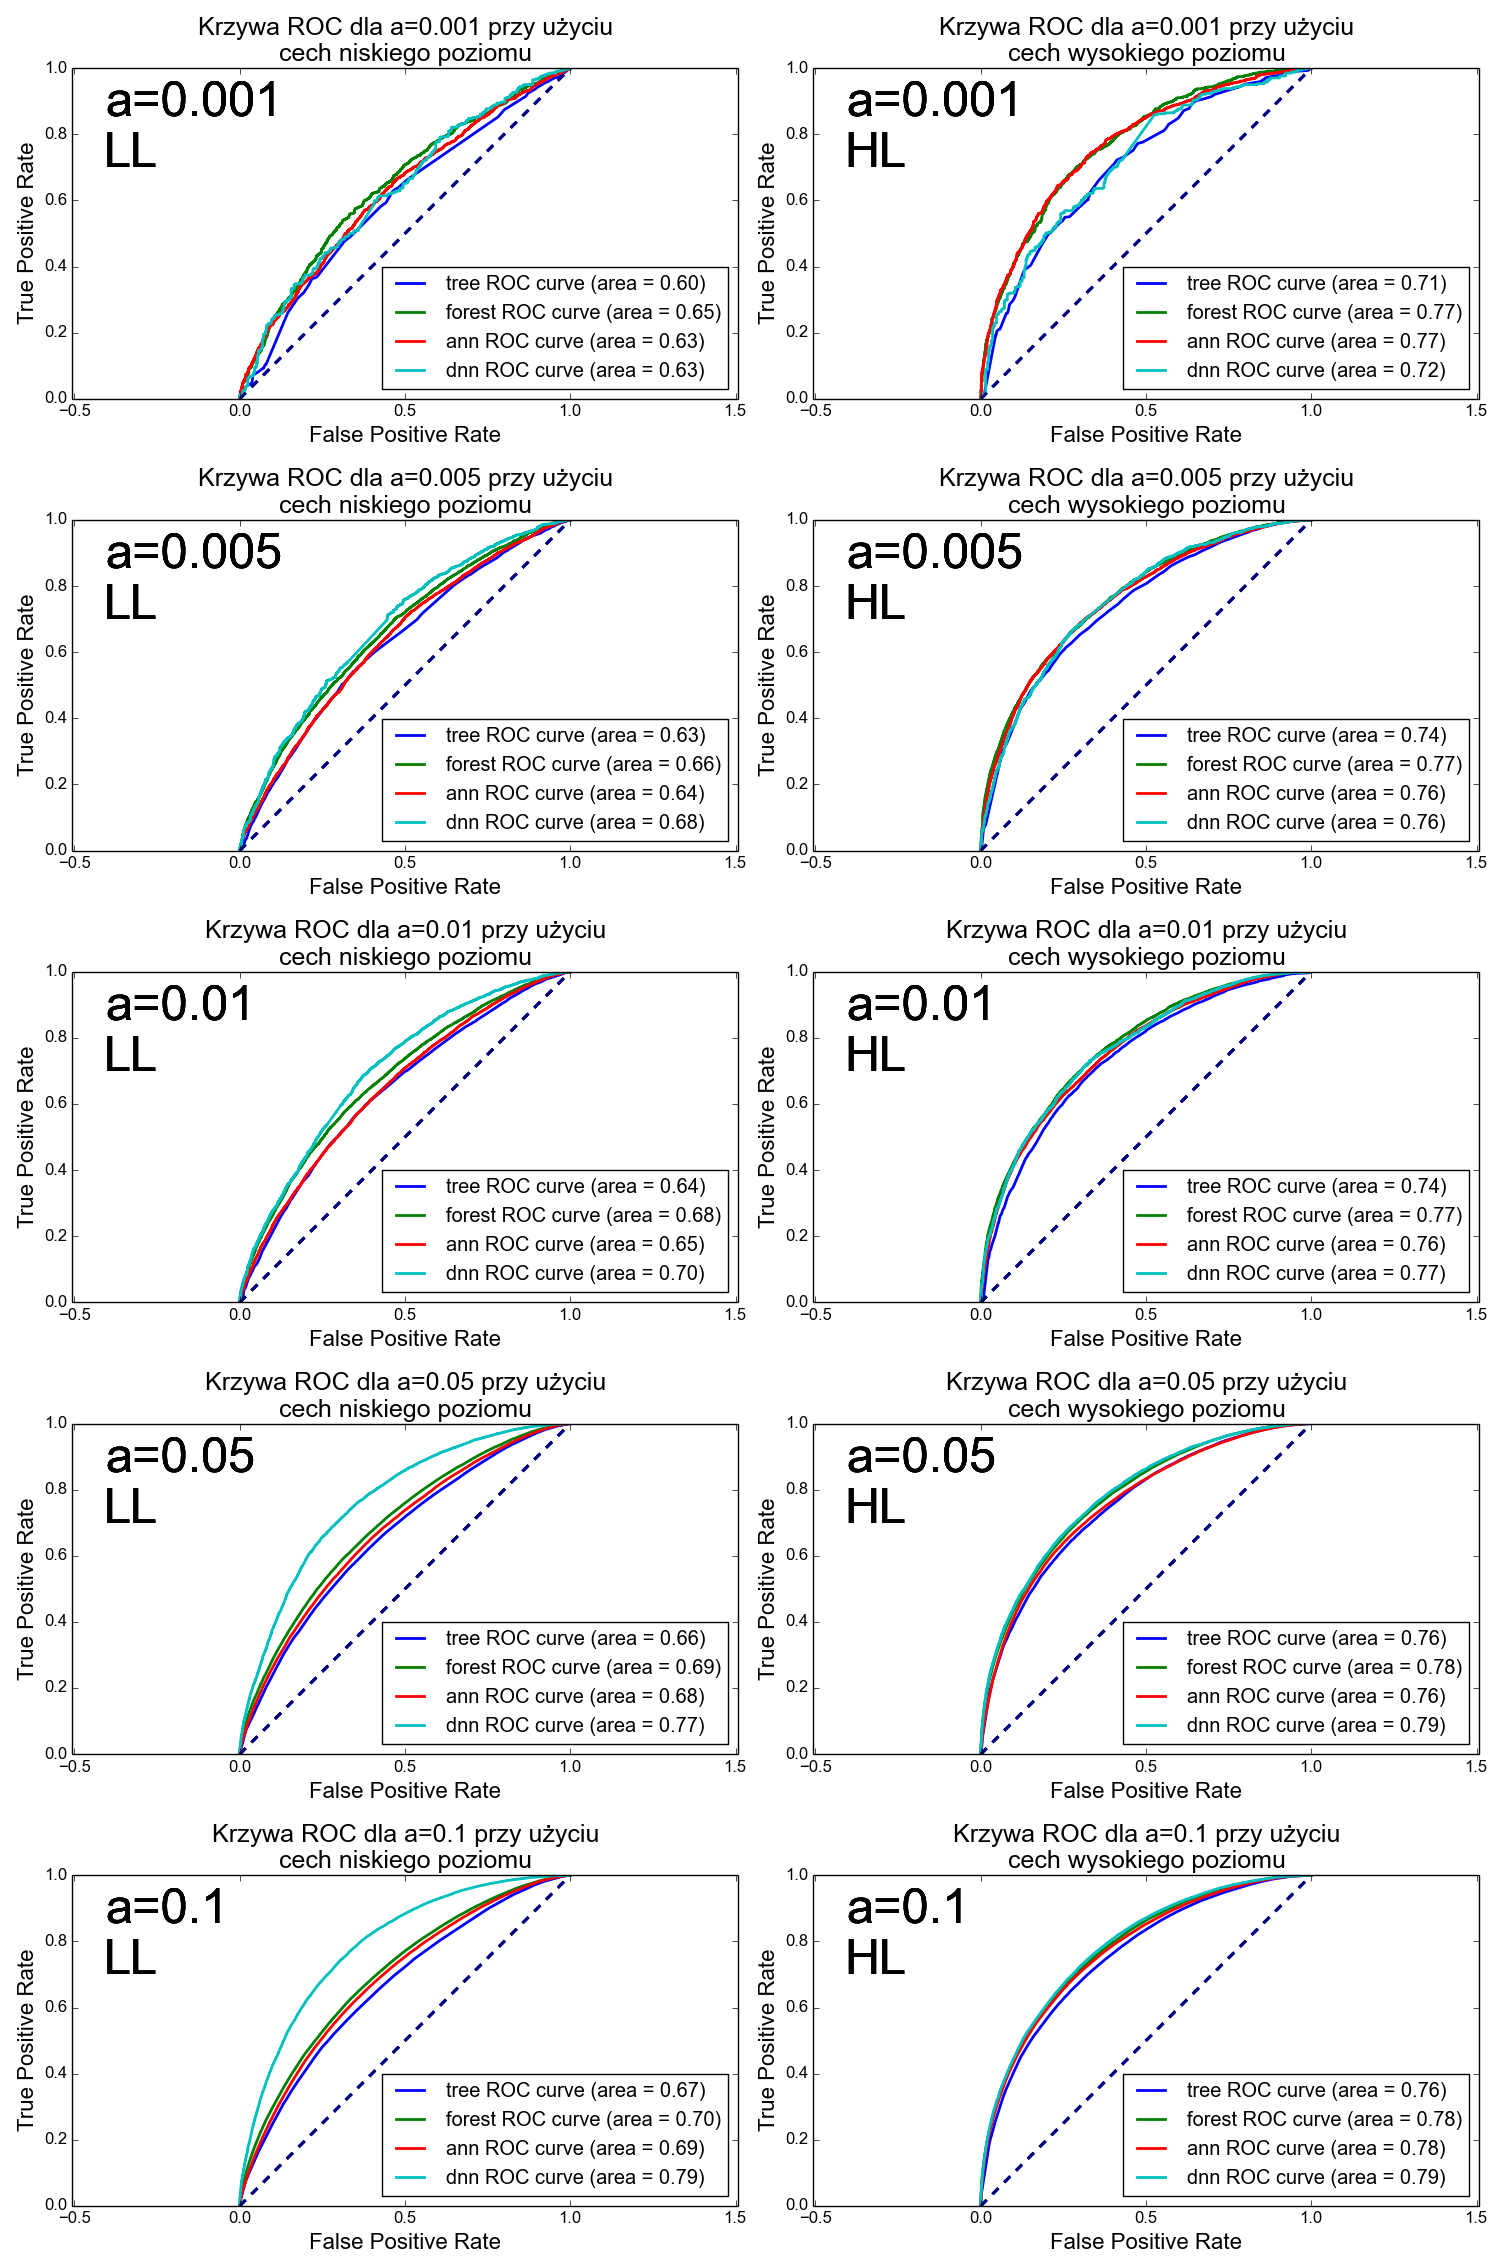
\includegraphics[scale=0.425]{res/allnew1.png}
\caption[Caption for LOF]{Krzywa ROC dla $a\in\{0.001, 0.005, 0.01, 0.05, 0.1\}$\label{higgsall1}}
\end{figure} 

\begin{figure}[ht!]
\centering
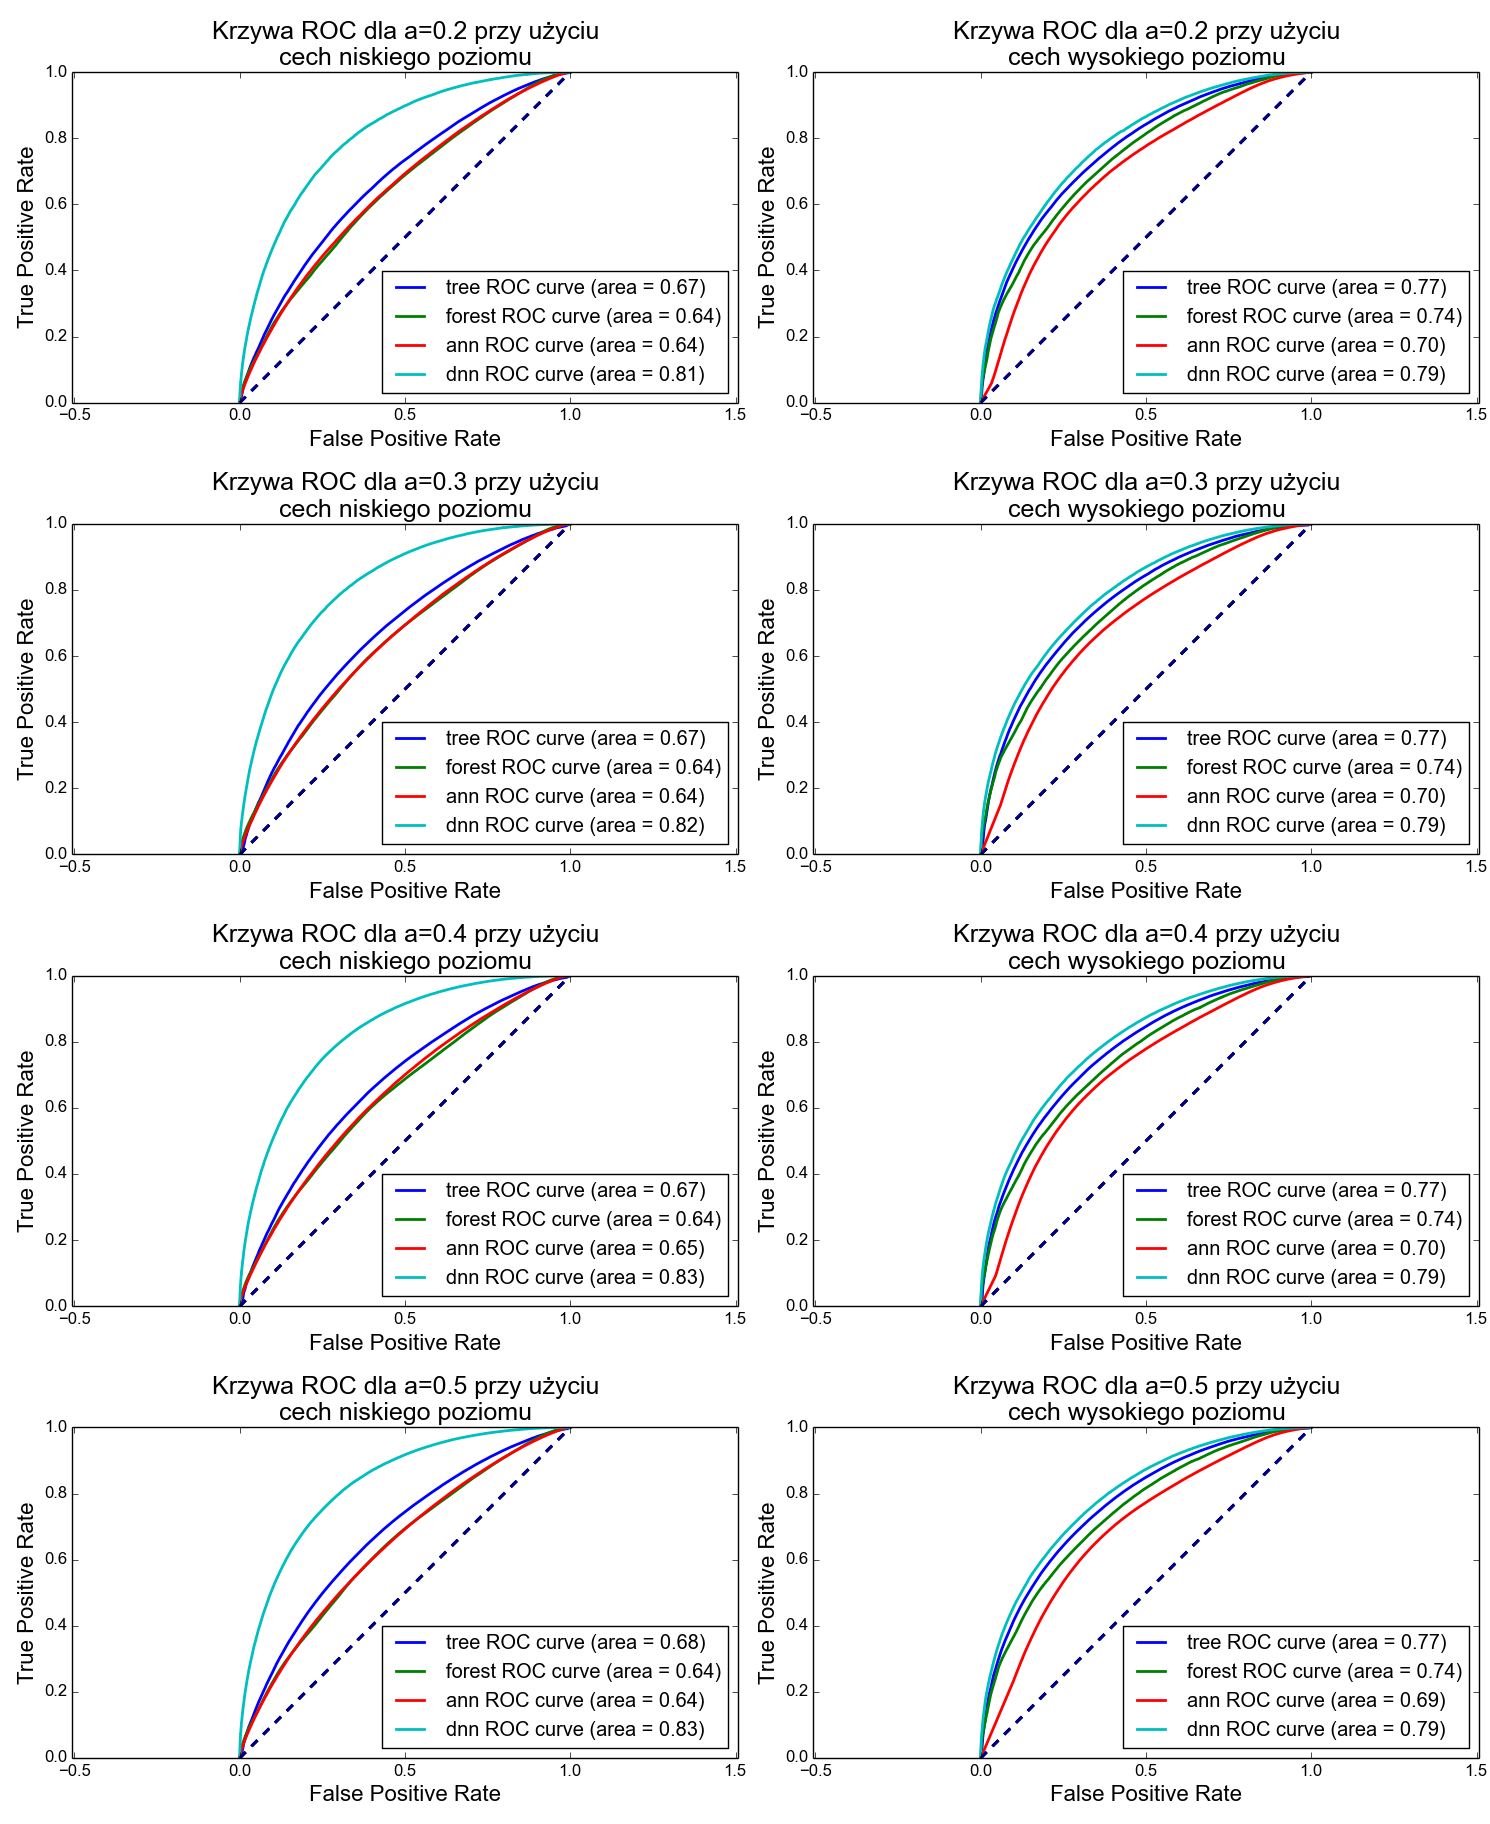
\includegraphics[scale=0.425]{res/allnew2.png}
\caption[Caption for LOF]{Krzywa ROC dla $a\in\{0.2, 0.3, 0.4, 0.5\}$\label{higgsall2}}
\end{figure} 

\begin{figure}[ht!]
\centering
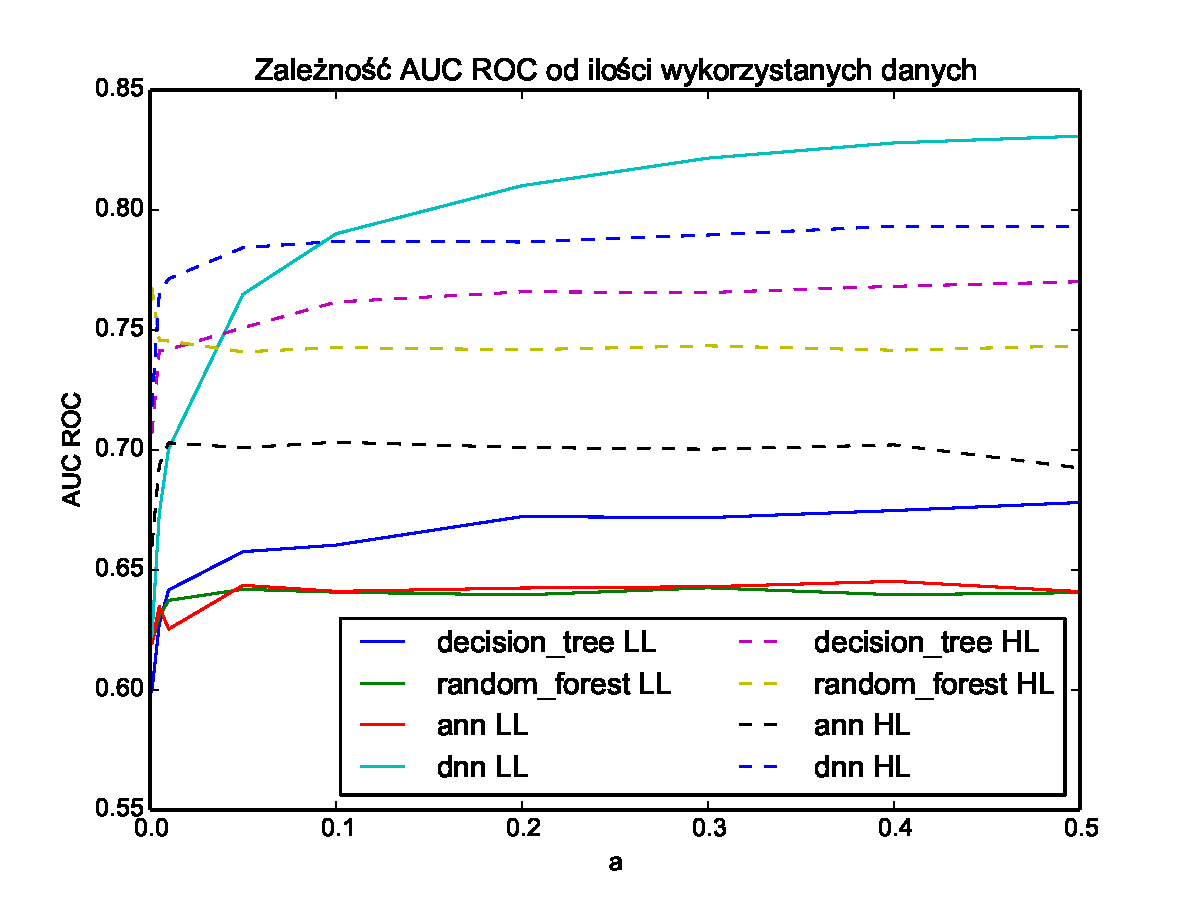
\includegraphics[scale=0.8]{res/higgssummary.pdf}
\caption[Caption for LOF]{Porównanie AUC ROC w zależności od rodzaju wykorzystanych cech dla wszystkich testowanych metod\label{higgssummary}}
\end{figure} 

\subsubsection{Wnioski}
Na~podstawie wykresu podsumowującego ten eksperyment, łatwo stwierdzić, że~w~przypadku wszystkich metod, przy użyciu mniejszej ilości danych uzyskane wyniki są znacznie lepsze w~przypadku wykorzystania cech wysokiego poziomu. Wraz ze~wzrostem liczby danych, skuteczność głębokich sieci neuronowych przy wykorzystaniu cech niskiego poziomu znacznie wzrasta i~szybko przewyższa wyniki innych metod niezależnie od~wykorzystanych atrybutów w~celu uczenia. W~przypadku, gdy $a=0.001$ najlepszy uzyskany wynik osiągnięty jest przy użyciu lasu drzew decyzyjnych (patrz tabela \ref{table:higgstable}). Stanowi to dowód na~to, że~w~przypadku niskiej liczby rekordów warto rozważyć ekstrakcje cech przy użyciu ,,wiedzy'' w~celu redukcji wymiarowości danych. Stwarza to możliwość użycia prostszych modeli uczenia maszynowego, które~są zdecydowanie łatwiejsze w~uczeniu w~przypadku, gdy dysponujemy niską ilością danych. Są one także bardziej odporne na~przeuczenie.


\section{Wnioski}

\clearpage
\addcontentsline{toc}{section}{Literatura}
\begingroup
\raggedright
\sloppy

\bibliography{bibliography}{}
\bibliographystyle{unsrt}

\endgroup
\renewcommand{\appendixtocname}{Dodatki}
\renewcommand{\appendixpagename}{Dodatki}

\clearpage

\begin{appendices}
\section{Obsługa programów}
Wszystkie stworzone programy umieszczone zostały w serwisie internetowym github.com. Dostęp do nich jest otwarty. Poniżej opisana została obsługa poszczególnych systemów.

\paragraph{System dotyczący sztucznego powielania danych}\mbox{}\\
Blabla

\paragraph{System dotyczący ekstrakcji cech przy pomocy metod matematycznych}\mbox{}\\
Blabla

\paragraph{System dotyczący ekstrakcji cech przy pomocy ,,wiedzy''}\mbox{}\\
Blabla

\paragraph{System dotyczący walidacji krzyżowej}\mbox{}\\
Blabla

\end{appendices}


\end{document}

%TODO:
% - podziekowania
% - polskie znaki
% - pojedyncze litery na koncu linii
% - spacje po kropce
% - footnotes na tej samej stronie
% \noindent